\documentclass[twoside]{book}

% Packages required by doxygen
\usepackage{calc}
\usepackage{doxygen}
\usepackage{graphicx}
\usepackage[utf8]{inputenc}
\usepackage{makeidx}
\usepackage{multicol}
\usepackage{multirow}
\usepackage{textcomp}
\usepackage[table]{xcolor}

% Font selection
\usepackage[T1]{fontenc}
\usepackage{mathptmx}
\usepackage[scaled=.90]{helvet}
\usepackage{courier}
\usepackage{amssymb}
\usepackage{sectsty}
\renewcommand{\familydefault}{\sfdefault}
\allsectionsfont{%
  \fontseries{bc}\selectfont%
  \color{darkgray}%
}
\renewcommand{\DoxyLabelFont}{%
  \fontseries{bc}\selectfont%
  \color{darkgray}%
}

% Page & text layout
\usepackage{geometry}
\geometry{%
  a4paper,%
  top=2.5cm,%
  bottom=2.5cm,%
  left=2.5cm,%
  right=2.5cm%
}
\tolerance=750
\hfuzz=15pt
\hbadness=750
\setlength{\emergencystretch}{15pt}
\setlength{\parindent}{0cm}
\setlength{\parskip}{0.2cm}
\makeatletter
\renewcommand{\paragraph}{%
  \@startsection{paragraph}{4}{0ex}{-1.0ex}{1.0ex}{%
    \normalfont\normalsize\bfseries\SS@parafont%
  }%
}
\renewcommand{\subparagraph}{%
  \@startsection{subparagraph}{5}{0ex}{-1.0ex}{1.0ex}{%
    \normalfont\normalsize\bfseries\SS@subparafont%
  }%
}
\makeatother

% Headers & footers
\usepackage{fancyhdr}
\pagestyle{fancyplain}
\fancyhead[LE]{\fancyplain{}{\bfseries\thepage}}
\fancyhead[CE]{\fancyplain{}{}}
\fancyhead[RE]{\fancyplain{}{\bfseries\leftmark}}
\fancyhead[LO]{\fancyplain{}{\bfseries\rightmark}}
\fancyhead[CO]{\fancyplain{}{}}
\fancyhead[RO]{\fancyplain{}{\bfseries\thepage}}
\fancyfoot[LE]{\fancyplain{}{}}
\fancyfoot[CE]{\fancyplain{}{}}
\fancyfoot[RE]{\fancyplain{}{\bfseries\scriptsize Generated on Mon Nov 11 2013 14\-:26\-:54 for My Project by Doxygen }}
\fancyfoot[LO]{\fancyplain{}{\bfseries\scriptsize Generated on Mon Nov 11 2013 14\-:26\-:54 for My Project by Doxygen }}
\fancyfoot[CO]{\fancyplain{}{}}
\fancyfoot[RO]{\fancyplain{}{}}
\renewcommand{\footrulewidth}{0.4pt}
\renewcommand{\chaptermark}[1]{%
  \markboth{#1}{}%
}
\renewcommand{\sectionmark}[1]{%
  \markright{\thesection\ #1}%
}

% Indices & bibliography
\usepackage{natbib}
\usepackage[titles]{tocloft}
\setcounter{tocdepth}{3}
\setcounter{secnumdepth}{5}
\makeindex

% Hyperlinks (required, but should be loaded last)
\usepackage{ifpdf}
\ifpdf
  \usepackage[pdftex,pagebackref=true]{hyperref}
\else
  \usepackage[ps2pdf,pagebackref=true]{hyperref}
\fi
\hypersetup{%
  colorlinks=true,%
  linkcolor=blue,%
  citecolor=blue,%
  unicode%
}

% Custom commands
\newcommand{\clearemptydoublepage}{%
  \newpage{\pagestyle{empty}\cleardoublepage}%
}


%===== C O N T E N T S =====

\begin{document}

% Titlepage & ToC
\hypersetup{pageanchor=false}
\pagenumbering{roman}
\begin{titlepage}
\vspace*{7cm}
\begin{center}%
{\Large My Project }\\
\vspace*{1cm}
{\large Generated by Doxygen 1.8.5}\\
\vspace*{0.5cm}
{\small Mon Nov 11 2013 14:26:54}\\
\end{center}
\end{titlepage}
\clearemptydoublepage
\tableofcontents
\clearemptydoublepage
\pagenumbering{arabic}
\hypersetup{pageanchor=true}

%--- Begin generated contents ---
\chapter{Hierarchical Index}
\section{Class Hierarchy}
This inheritance list is sorted roughly, but not completely, alphabetically\-:\begin{DoxyCompactList}
\item C\-C\-Application\begin{DoxyCompactList}
\item \contentsline{section}{App\-Delegate}{\pageref{class_app_delegate}}{}
\end{DoxyCompactList}
\item C\-C\-Layer\begin{DoxyCompactList}
\item \contentsline{section}{J\-G\-\_\-\-Main\-\_\-\-Game}{\pageref{class_j_g___main___game}}{}
\item \contentsline{section}{J\-G\-\_\-\-Main\-\_\-\-Menu}{\pageref{class_j_g___main___menu}}{}
\end{DoxyCompactList}
\item C\-C\-Node\begin{DoxyCompactList}
\item \contentsline{section}{J\-G\-\_\-\-Temp\-Line\-Container}{\pageref{class_j_g___temp_line_container}}{}
\end{DoxyCompactList}
\item C\-C\-Sprite\begin{DoxyCompactList}
\item \contentsline{section}{J\-G\-\_\-\-Ball}{\pageref{class_j_g___ball}}{}
\item \contentsline{section}{J\-G\-\_\-\-Bonus\-\_\-\-Base}{\pageref{class_j_g___bonus___base}}{}
\item \contentsline{section}{J\-G\-\_\-\-Hand}{\pageref{class_j_g___hand}}{}
\end{DoxyCompactList}
\end{DoxyCompactList}

\chapter{Class Index}
\section{Class List}
Here are the classes, structs, unions and interfaces with brief descriptions\-:\begin{DoxyCompactList}
\item\contentsline{section}{\hyperlink{class_app_delegate}{App\-Delegate} }{\pageref{class_app_delegate}}{}
\item\contentsline{section}{\hyperlink{class_j_g___ball}{J\-G\-\_\-\-Ball} }{\pageref{class_j_g___ball}}{}
\item\contentsline{section}{\hyperlink{class_j_g___bonus___base}{J\-G\-\_\-\-Bonus\-\_\-\-Base} }{\pageref{class_j_g___bonus___base}}{}
\item\contentsline{section}{\hyperlink{class_j_g___game___h_u_d}{J\-G\-\_\-\-Game\-\_\-\-H\-U\-D} }{\pageref{class_j_g___game___h_u_d}}{}
\item\contentsline{section}{\hyperlink{class_j_g___game___main}{J\-G\-\_\-\-Game\-\_\-\-Main} }{\pageref{class_j_g___game___main}}{}
\item\contentsline{section}{\hyperlink{class_j_g___hand}{J\-G\-\_\-\-Hand} }{\pageref{class_j_g___hand}}{}
\item\contentsline{section}{\hyperlink{class_j_g___menu___main}{J\-G\-\_\-\-Menu\-\_\-\-Main} }{\pageref{class_j_g___menu___main}}{}
\item\contentsline{section}{\hyperlink{struct_s_touch_info}{S\-Touch\-Info} }{\pageref{struct_s_touch_info}}{}
\item\contentsline{section}{\hyperlink{structtag_resource}{tag\-Resource} \\*The cocos2d Application }{\pageref{structtag_resource}}{}
\end{DoxyCompactList}

\chapter{Class Documentation}
\hypertarget{class_app_delegate}{\section{App\-Delegate Class Reference}
\label{class_app_delegate}\index{App\-Delegate@{App\-Delegate}}
}
Inheritance diagram for App\-Delegate\-:\begin{figure}[H]
\begin{center}
\leavevmode
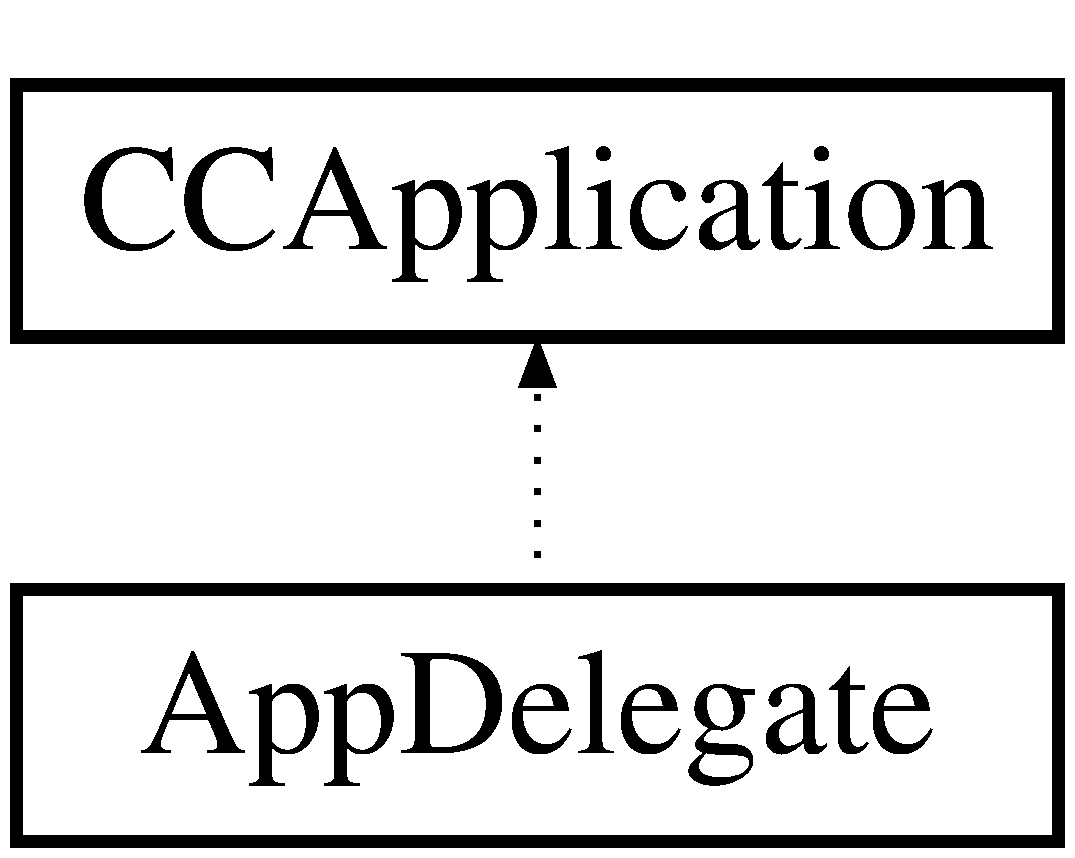
\includegraphics[height=2.000000cm]{class_app_delegate}
\end{center}
\end{figure}
\subsection*{Public Member Functions}
\begin{DoxyCompactItemize}
\item 
virtual bool \hyperlink{class_app_delegate_a68cbaed49edf7581dc59a09d5062fff3}{application\-Did\-Finish\-Launching} ()
\begin{DoxyCompactList}\small\item\em Implement C\-C\-Director and C\-C\-Scene init code here. \end{DoxyCompactList}\item 
virtual void \hyperlink{class_app_delegate_a17cb09777419781698324e0415bffd3a}{application\-Did\-Enter\-Background} ()
\begin{DoxyCompactList}\small\item\em The function be called when the application enter background. \end{DoxyCompactList}\item 
virtual void \hyperlink{class_app_delegate_ac4d653e3f74a91efef5f2def58fe3108}{application\-Will\-Enter\-Foreground} ()
\begin{DoxyCompactList}\small\item\em The function be called when the application enter foreground. \end{DoxyCompactList}\end{DoxyCompactItemize}


\subsection{Member Function Documentation}
\hypertarget{class_app_delegate_a17cb09777419781698324e0415bffd3a}{\index{App\-Delegate@{App\-Delegate}!application\-Did\-Enter\-Background@{application\-Did\-Enter\-Background}}
\index{application\-Did\-Enter\-Background@{application\-Did\-Enter\-Background}!AppDelegate@{App\-Delegate}}
\subsubsection[{application\-Did\-Enter\-Background}]{\setlength{\rightskip}{0pt plus 5cm}void App\-Delegate\-::application\-Did\-Enter\-Background (
\begin{DoxyParamCaption}
{}
\end{DoxyParamCaption}
)\hspace{0.3cm}{\ttfamily [virtual]}}}\label{class_app_delegate_a17cb09777419781698324e0415bffd3a}


The function be called when the application enter background. 


\begin{DoxyParams}{Parameters}
{\em the} & pointer of the application \\
\hline
\end{DoxyParams}
\hypertarget{class_app_delegate_a68cbaed49edf7581dc59a09d5062fff3}{\index{App\-Delegate@{App\-Delegate}!application\-Did\-Finish\-Launching@{application\-Did\-Finish\-Launching}}
\index{application\-Did\-Finish\-Launching@{application\-Did\-Finish\-Launching}!AppDelegate@{App\-Delegate}}
\subsubsection[{application\-Did\-Finish\-Launching}]{\setlength{\rightskip}{0pt plus 5cm}bool App\-Delegate\-::application\-Did\-Finish\-Launching (
\begin{DoxyParamCaption}
{}
\end{DoxyParamCaption}
)\hspace{0.3cm}{\ttfamily [virtual]}}}\label{class_app_delegate_a68cbaed49edf7581dc59a09d5062fff3}


Implement C\-C\-Director and C\-C\-Scene init code here. 

\begin{DoxyReturn}{Returns}
true Initialize success, app continue. 

false Initialize failed, app terminate. 
\end{DoxyReturn}
\hypertarget{class_app_delegate_ac4d653e3f74a91efef5f2def58fe3108}{\index{App\-Delegate@{App\-Delegate}!application\-Will\-Enter\-Foreground@{application\-Will\-Enter\-Foreground}}
\index{application\-Will\-Enter\-Foreground@{application\-Will\-Enter\-Foreground}!AppDelegate@{App\-Delegate}}
\subsubsection[{application\-Will\-Enter\-Foreground}]{\setlength{\rightskip}{0pt plus 5cm}void App\-Delegate\-::application\-Will\-Enter\-Foreground (
\begin{DoxyParamCaption}
{}
\end{DoxyParamCaption}
)\hspace{0.3cm}{\ttfamily [virtual]}}}\label{class_app_delegate_ac4d653e3f74a91efef5f2def58fe3108}


The function be called when the application enter foreground. 


\begin{DoxyParams}{Parameters}
{\em the} & pointer of the application \\
\hline
\end{DoxyParams}


The documentation for this class was generated from the following files\-:\begin{DoxyCompactItemize}
\item 
App\-Delegate.\-h\item 
App\-Delegate.\-cpp\end{DoxyCompactItemize}

\hypertarget{class_j_g___ball}{\section{J\-G\-\_\-\-Ball Class Reference}
\label{class_j_g___ball}\index{J\-G\-\_\-\-Ball@{J\-G\-\_\-\-Ball}}
}


{\ttfamily \#include $<$J\-G\-\_\-\-Ball.\-h$>$}

Inheritance diagram for J\-G\-\_\-\-Ball\-:\begin{figure}[H]
\begin{center}
\leavevmode
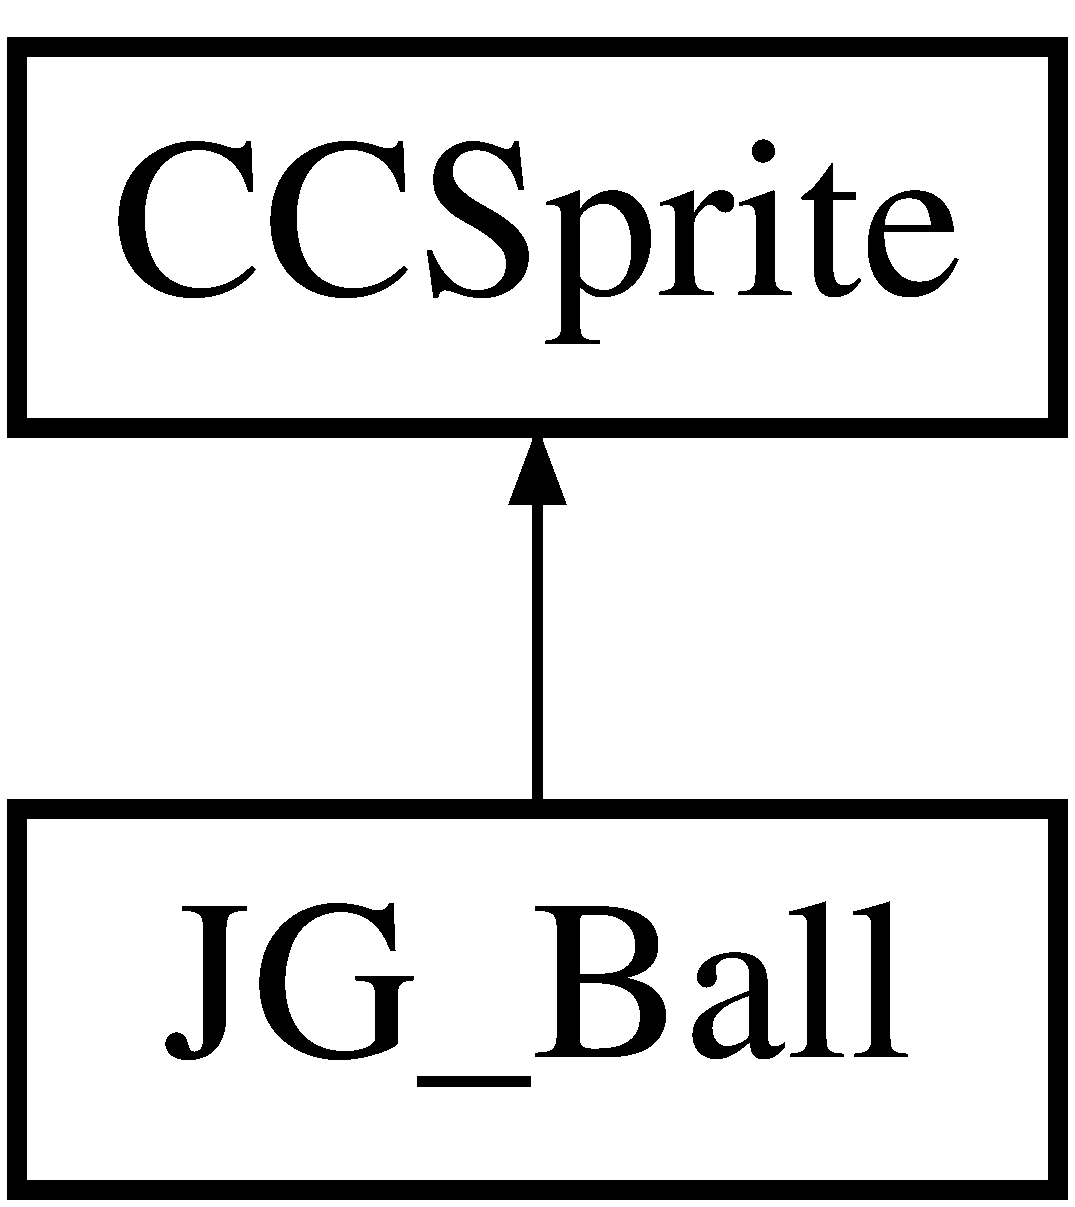
\includegraphics[height=2.000000cm]{class_j_g___ball}
\end{center}
\end{figure}
\subsection*{Public Member Functions}
\begin{DoxyCompactItemize}
\item 
void \hyperlink{class_j_g___ball_a601eda0b1aaf9d4c8fdd31d36234a6c1}{Move\-Curve} (float force, C\-C\-Point destination)
\item 
void \hyperlink{class_j_g___ball_afa347dae4a20695cf506375b798cb2f3}{Move\-Staight} (float force, C\-C\-Point destination)
\item 
void \hyperlink{class_j_g___ball_a21c06d1a10aa8fdcc3d8e63a82f221fe}{update} (float dt)
\item 
\hypertarget{class_j_g___ball_adb4350ed0da24e5499c3402bc322f559}{void {\bfseries temp\-Reset} ()}\label{class_j_g___ball_adb4350ed0da24e5499c3402bc322f559}

\item 
E\-Throw\-Direction \hyperlink{class_j_g___ball_a94843b91ab6f8cddbb2b90de6daeb531}{Get\-Ball\-Direction} ()
\item 
\hypertarget{class_j_g___ball_a0ad42506b43718f14ccb45f163d92999}{C\-C\-Point {\bfseries Get\-Initial\-Touch\-Position} ()}\label{class_j_g___ball_a0ad42506b43718f14ccb45f163d92999}

\item 
\hypertarget{class_j_g___ball_a628e6f457315f1af9d9638834dff91e0}{void {\bfseries Set\-Initial\-Touch\-Position} (C\-C\-Point new\-Touch\-Pos)}\label{class_j_g___ball_a628e6f457315f1af9d9638834dff91e0}

\end{DoxyCompactItemize}
\subsection*{Static Public Member Functions}
\begin{DoxyCompactItemize}
\item 
static \hyperlink{class_j_g___ball}{J\-G\-\_\-\-Ball} $\ast$ \hyperlink{class_j_g___ball_a12279a500446c9516026d3f52fee87eb}{create\-With\-File\-Name} (const char $\ast$psz\-File\-Name, C\-C\-Point initial\-Pos)
\item 
static void \hyperlink{class_j_g___ball_a8023f3c38c257dd4430a5a01c519a289}{Calculate\-Speed\-Boundries\-Base\-On\-Length} (float delta\-X)
\end{DoxyCompactItemize}
\subsection*{Public Attributes}
\begin{DoxyCompactItemize}
\item 
\hypertarget{class_j_g___ball_ad4aa2855022e5315addf40ef73ee6972}{float {\bfseries speed}}\label{class_j_g___ball_ad4aa2855022e5315addf40ef73ee6972}

\item 
\hypertarget{class_j_g___ball_a743ed73473f38e9466f305c3f8efe995}{E\-Throw\-Direction {\bfseries ball\-Throw\-Direction}}\label{class_j_g___ball_a743ed73473f38e9466f305c3f8efe995}

\item 
\hypertarget{class_j_g___ball_af0bd7eeacc5d8f094d921663843b5179}{float {\bfseries curve\-\_\-\-Total\-Time}}\label{class_j_g___ball_af0bd7eeacc5d8f094d921663843b5179}

\item 
\hypertarget{class_j_g___ball_a681ecc9587d2d8d857f656d19d297ef8}{float {\bfseries curve\-\_\-\-Y0}}\label{class_j_g___ball_a681ecc9587d2d8d857f656d19d297ef8}

\item 
\hypertarget{class_j_g___ball_a8dcbff9b6d7f9f8737b3421f26c699e7}{float {\bfseries curve\-\_\-\-X0}}\label{class_j_g___ball_a8dcbff9b6d7f9f8737b3421f26c699e7}

\item 
\hypertarget{class_j_g___ball_a32222cd24992fff289361884db472b23}{float {\bfseries curve\-\_\-\-Rad}}\label{class_j_g___ball_a32222cd24992fff289361884db472b23}

\item 
\hypertarget{class_j_g___ball_a399ae1fb026df3759d3616c7b74eecaa}{float {\bfseries straight\-\_\-\-Dir}}\label{class_j_g___ball_a399ae1fb026df3759d3616c7b74eecaa}

\item 
\hypertarget{class_j_g___ball_a2cab0645b2eb4374fbfde0b0399c0e72}{C\-C\-Point {\bfseries temp\-Initial\-Position}}\label{class_j_g___ball_a2cab0645b2eb4374fbfde0b0399c0e72}

\item 
\hypertarget{class_j_g___ball_a358259dea815fa262327e0af48a6af3c}{E\-Throw\-Direction {\bfseries temp\-Initial\-Throw\-Direction}}\label{class_j_g___ball_a358259dea815fa262327e0af48a6af3c}

\item 
\hypertarget{class_j_g___ball_a602558390080ce6d8cdfcfdbc09f7b12}{C\-C\-Repeat\-Forever $\ast$ {\bfseries action\-\_\-\-Rotate}}\label{class_j_g___ball_a602558390080ce6d8cdfcfdbc09f7b12}

\item 
\hypertarget{class_j_g___ball_aa0fc27312d724fcf2324e87844a99cb8}{\hyperlink{class_j_g___temp_line_container}{J\-G\-\_\-\-Temp\-Line\-Container} $\ast$ {\bfseries temp\-Draw}}\label{class_j_g___ball_aa0fc27312d724fcf2324e87844a99cb8}

\item 
\hypertarget{class_j_g___ball_aacc0e044d12a3fe88d03b54f8c800626}{C\-C\-Point {\bfseries touch\-Position}}\label{class_j_g___ball_aacc0e044d12a3fe88d03b54f8c800626}

\item 
\hypertarget{class_j_g___ball_a0ad0f2f4b8d03d63c879544111a24506}{E\-Move\-Mode {\bfseries move\-Mode}}\label{class_j_g___ball_a0ad0f2f4b8d03d63c879544111a24506}

\end{DoxyCompactItemize}
\subsection*{Static Public Attributes}
\begin{DoxyCompactItemize}
\item 
\hypertarget{class_j_g___ball_a0e5845ccdb93030b567b796f6266e517}{static float {\bfseries min\-Speed}}\label{class_j_g___ball_a0e5845ccdb93030b567b796f6266e517}

\item 
\hypertarget{class_j_g___ball_ad830251662cdf8443962aef638ffefcc}{static float {\bfseries max\-Speed}}\label{class_j_g___ball_ad830251662cdf8443962aef638ffefcc}

\end{DoxyCompactItemize}


\subsection{Detailed Description}
class for handling ball 

\subsection{Member Function Documentation}
\hypertarget{class_j_g___ball_a8023f3c38c257dd4430a5a01c519a289}{\index{J\-G\-\_\-\-Ball@{J\-G\-\_\-\-Ball}!Calculate\-Speed\-Boundries\-Base\-On\-Length@{Calculate\-Speed\-Boundries\-Base\-On\-Length}}
\index{Calculate\-Speed\-Boundries\-Base\-On\-Length@{Calculate\-Speed\-Boundries\-Base\-On\-Length}!JG_Ball@{J\-G\-\_\-\-Ball}}
\subsubsection[{Calculate\-Speed\-Boundries\-Base\-On\-Length}]{\setlength{\rightskip}{0pt plus 5cm}static void J\-G\-\_\-\-Ball\-::\-Calculate\-Speed\-Boundries\-Base\-On\-Length (
\begin{DoxyParamCaption}
\item[{float}]{delta\-X}
\end{DoxyParamCaption}
)\hspace{0.3cm}{\ttfamily [inline]}, {\ttfamily [static]}}}\label{class_j_g___ball_a8023f3c38c257dd4430a5a01c519a289}
Calculate the minimum Speed , based on the distance of handes \hypertarget{class_j_g___ball_a12279a500446c9516026d3f52fee87eb}{\index{J\-G\-\_\-\-Ball@{J\-G\-\_\-\-Ball}!create\-With\-File\-Name@{create\-With\-File\-Name}}
\index{create\-With\-File\-Name@{create\-With\-File\-Name}!JG_Ball@{J\-G\-\_\-\-Ball}}
\subsubsection[{create\-With\-File\-Name}]{\setlength{\rightskip}{0pt plus 5cm}{\bf J\-G\-\_\-\-Ball} $\ast$ J\-G\-\_\-\-Ball\-::create\-With\-File\-Name (
\begin{DoxyParamCaption}
\item[{const char $\ast$}]{psz\-File\-Name, }
\item[{C\-C\-Point}]{initial\-Pos}
\end{DoxyParamCaption}
)\hspace{0.3cm}{\ttfamily [static]}}}\label{class_j_g___ball_a12279a500446c9516026d3f52fee87eb}
Creating ball in a specific position \hypertarget{class_j_g___ball_a94843b91ab6f8cddbb2b90de6daeb531}{\index{J\-G\-\_\-\-Ball@{J\-G\-\_\-\-Ball}!Get\-Ball\-Direction@{Get\-Ball\-Direction}}
\index{Get\-Ball\-Direction@{Get\-Ball\-Direction}!JG_Ball@{J\-G\-\_\-\-Ball}}
\subsubsection[{Get\-Ball\-Direction}]{\setlength{\rightskip}{0pt plus 5cm}E\-Throw\-Direction J\-G\-\_\-\-Ball\-::\-Get\-Ball\-Direction (
\begin{DoxyParamCaption}
{}
\end{DoxyParamCaption}
)\hspace{0.3cm}{\ttfamily [inline]}}}\label{class_j_g___ball_a94843b91ab6f8cddbb2b90de6daeb531}
get the direction of ball \hypertarget{class_j_g___ball_a601eda0b1aaf9d4c8fdd31d36234a6c1}{\index{J\-G\-\_\-\-Ball@{J\-G\-\_\-\-Ball}!Move\-Curve@{Move\-Curve}}
\index{Move\-Curve@{Move\-Curve}!JG_Ball@{J\-G\-\_\-\-Ball}}
\subsubsection[{Move\-Curve}]{\setlength{\rightskip}{0pt plus 5cm}void J\-G\-\_\-\-Ball\-::\-Move\-Curve (
\begin{DoxyParamCaption}
\item[{float}]{force, }
\item[{C\-C\-Point}]{destination}
\end{DoxyParamCaption}
)}}\label{class_j_g___ball_a601eda0b1aaf9d4c8fdd31d36234a6c1}
Initial the curve movement variables \hypertarget{class_j_g___ball_afa347dae4a20695cf506375b798cb2f3}{\index{J\-G\-\_\-\-Ball@{J\-G\-\_\-\-Ball}!Move\-Staight@{Move\-Staight}}
\index{Move\-Staight@{Move\-Staight}!JG_Ball@{J\-G\-\_\-\-Ball}}
\subsubsection[{Move\-Staight}]{\setlength{\rightskip}{0pt plus 5cm}void J\-G\-\_\-\-Ball\-::\-Move\-Staight (
\begin{DoxyParamCaption}
\item[{float}]{force, }
\item[{C\-C\-Point}]{destination}
\end{DoxyParamCaption}
)}}\label{class_j_g___ball_afa347dae4a20695cf506375b798cb2f3}
Initial the straight movement variables \hypertarget{class_j_g___ball_a21c06d1a10aa8fdcc3d8e63a82f221fe}{\index{J\-G\-\_\-\-Ball@{J\-G\-\_\-\-Ball}!update@{update}}
\index{update@{update}!JG_Ball@{J\-G\-\_\-\-Ball}}
\subsubsection[{update}]{\setlength{\rightskip}{0pt plus 5cm}void J\-G\-\_\-\-Ball\-::update (
\begin{DoxyParamCaption}
\item[{float}]{dt}
\end{DoxyParamCaption}
)}}\label{class_j_g___ball_a21c06d1a10aa8fdcc3d8e63a82f221fe}
Handles the movement based on the current mode 

The documentation for this class was generated from the following files\-:\begin{DoxyCompactItemize}
\item 
J\-G\-\_\-\-Ball.\-h\item 
J\-G\-\_\-\-Ball.\-cpp\end{DoxyCompactItemize}

\hypertarget{class_j_g___bonus___base}{\section{J\-G\-\_\-\-Bonus\-\_\-\-Base Class Reference}
\label{class_j_g___bonus___base}\index{J\-G\-\_\-\-Bonus\-\_\-\-Base@{J\-G\-\_\-\-Bonus\-\_\-\-Base}}
}
Inheritance diagram for J\-G\-\_\-\-Bonus\-\_\-\-Base\-:\begin{figure}[H]
\begin{center}
\leavevmode
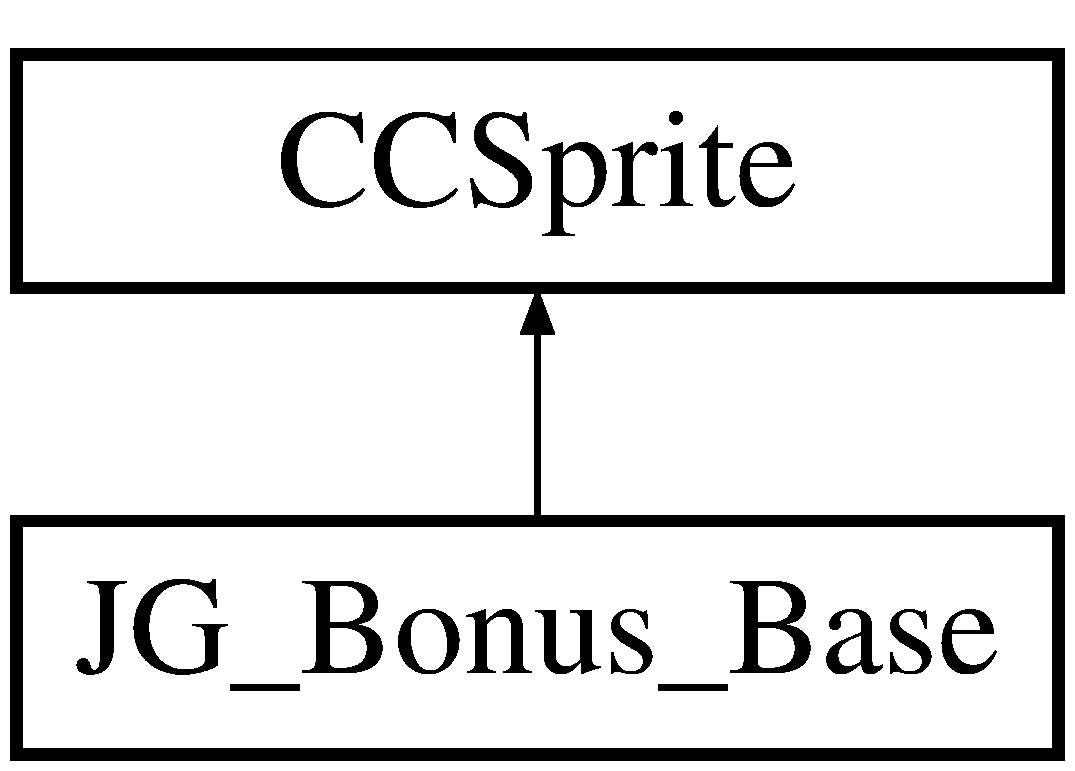
\includegraphics[height=2.000000cm]{class_j_g___bonus___base}
\end{center}
\end{figure}


The documentation for this class was generated from the following files\-:\begin{DoxyCompactItemize}
\item 
J\-G\-\_\-\-Bonus\-\_\-\-Base.\-h\item 
J\-G\-\_\-\-Bonus\-\_\-\-Base.\-cpp\end{DoxyCompactItemize}

\hypertarget{class_j_g___game___h_u_d}{\section{J\-G\-\_\-\-Game\-\_\-\-H\-U\-D Class Reference}
\label{class_j_g___game___h_u_d}\index{J\-G\-\_\-\-Game\-\_\-\-H\-U\-D@{J\-G\-\_\-\-Game\-\_\-\-H\-U\-D}}
}
Inheritance diagram for J\-G\-\_\-\-Game\-\_\-\-H\-U\-D\-:\begin{figure}[H]
\begin{center}
\leavevmode
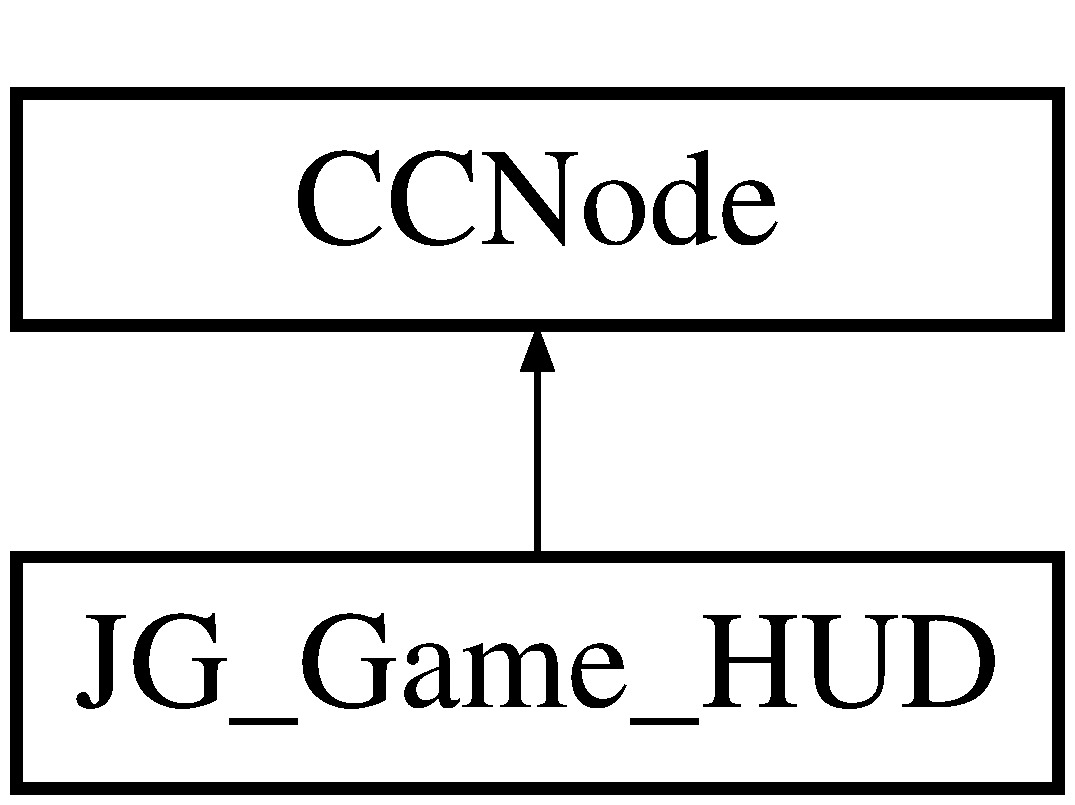
\includegraphics[height=2.000000cm]{class_j_g___game___h_u_d}
\end{center}
\end{figure}
\subsection*{Public Member Functions}
\begin{DoxyCompactItemize}
\item 
\hypertarget{class_j_g___game___h_u_d_aef2a88064a176f3d621da7a51f3a534d}{bool {\bfseries init} (\hyperlink{class_j_g___game___main}{J\-G\-\_\-\-Game\-\_\-\-Main} $\ast$game)}\label{class_j_g___game___h_u_d_aef2a88064a176f3d621da7a51f3a534d}

\item 
\hypertarget{class_j_g___game___h_u_d_a9d7347316f245e90d914e60da1138e14}{void {\bfseries Init\-\_\-\-Pause\-Menu} ()}\label{class_j_g___game___h_u_d_a9d7347316f245e90d914e60da1138e14}

\item 
\hypertarget{class_j_g___game___h_u_d_aafd38bbdaf7e8e2b5111be32b932adca}{void {\bfseries Set\-Pause\-Screen} (bool b\-Show)}\label{class_j_g___game___h_u_d_aafd38bbdaf7e8e2b5111be32b932adca}

\item 
\hypertarget{class_j_g___game___h_u_d_af65407785d15c72c92fb4cf4df54cae3}{void {\bfseries draw} ()}\label{class_j_g___game___h_u_d_af65407785d15c72c92fb4cf4df54cae3}

\item 
\hypertarget{class_j_g___game___h_u_d_ae1d35126fa37a9647365bdb96402a388}{void {\bfseries Draw\-Life} ()}\label{class_j_g___game___h_u_d_ae1d35126fa37a9647365bdb96402a388}

\item 
\hypertarget{class_j_g___game___h_u_d_ad7b8a1d0920dc3abb928eb6705c03efe}{void {\bfseries Update\-Score} ()}\label{class_j_g___game___h_u_d_ad7b8a1d0920dc3abb928eb6705c03efe}

\end{DoxyCompactItemize}
\subsection*{Static Public Member Functions}
\begin{DoxyCompactItemize}
\item 
\hypertarget{class_j_g___game___h_u_d_aa4c8aae108b41d13fdd5480abc34a595}{static \hyperlink{class_j_g___game___h_u_d}{J\-G\-\_\-\-Game\-\_\-\-H\-U\-D} $\ast$ {\bfseries create} (\hyperlink{class_j_g___game___main}{J\-G\-\_\-\-Game\-\_\-\-Main} $\ast$game)}\label{class_j_g___game___h_u_d_aa4c8aae108b41d13fdd5480abc34a595}

\end{DoxyCompactItemize}
\subsection*{Public Attributes}
\begin{DoxyCompactItemize}
\item 
\hypertarget{class_j_g___game___h_u_d_ade165083e41d5e1a33471824593ea825}{C\-C\-Sprite $\ast$ {\bfseries game\-Reset\-Sprite\-\_\-\-On}}\label{class_j_g___game___h_u_d_ade165083e41d5e1a33471824593ea825}

\item 
\hypertarget{class_j_g___game___h_u_d_aaa968d54de47be33bc87c132c6e390a3}{C\-C\-Sprite $\ast$ {\bfseries game\-Reset\-Sprite\-\_\-\-Off}}\label{class_j_g___game___h_u_d_aaa968d54de47be33bc87c132c6e390a3}

\item 
\hypertarget{class_j_g___game___h_u_d_ac314377862b92a8215aedc417ddbfe34}{C\-C\-Menu\-Item\-Sprite $\ast$ {\bfseries pause\-Button}}\label{class_j_g___game___h_u_d_ac314377862b92a8215aedc417ddbfe34}

\item 
\hypertarget{class_j_g___game___h_u_d_aa0c12912c381303ba392097b1a9dd0ba}{C\-C\-Menu\-Item\-Sprite $\ast$ {\bfseries reset\-Button}}\label{class_j_g___game___h_u_d_aa0c12912c381303ba392097b1a9dd0ba}

\item 
\hypertarget{class_j_g___game___h_u_d_ae55dc5788c420fefbe77de5ce15de48e}{C\-C\-Menu\-Item\-Sprite $\ast$ {\bfseries resume\-Button}}\label{class_j_g___game___h_u_d_ae55dc5788c420fefbe77de5ce15de48e}

\item 
\hypertarget{class_j_g___game___h_u_d_ac19bdb8355802968b5397d060d0ac5a6}{C\-C\-Menu\-Item\-Sprite $\ast$ {\bfseries exit\-Button}}\label{class_j_g___game___h_u_d_ac19bdb8355802968b5397d060d0ac5a6}

\item 
\hypertarget{class_j_g___game___h_u_d_af1c1b7a1e1664b6f228e0ac2af1a90f8}{C\-C\-Menu $\ast$ {\bfseries game\-Menu}}\label{class_j_g___game___h_u_d_af1c1b7a1e1664b6f228e0ac2af1a90f8}

\item 
\hypertarget{class_j_g___game___h_u_d_a0fa6c42a04e522b4be2e3f9ec3a4c086}{C\-C\-Point {\bfseries life\-Draw\-Position}}\label{class_j_g___game___h_u_d_a0fa6c42a04e522b4be2e3f9ec3a4c086}

\item 
\hypertarget{class_j_g___game___h_u_d_a5d3beeabb044da9cbdf09d51dd5579c3}{int {\bfseries life\-Draw\-Pacing}}\label{class_j_g___game___h_u_d_a5d3beeabb044da9cbdf09d51dd5579c3}

\item 
\hypertarget{class_j_g___game___h_u_d_a2bb9f6ccfa05f75a13c0e87eab0cb31d}{C\-C\-Texture2\-D $\ast$ {\bfseries life\-Texture\-\_\-\-Active}}\label{class_j_g___game___h_u_d_a2bb9f6ccfa05f75a13c0e87eab0cb31d}

\item 
\hypertarget{class_j_g___game___h_u_d_a30f9f7a663ee085f9e7395baf2f84f1d}{C\-C\-Texture2\-D $\ast$ {\bfseries life\-Texture\-\_\-\-Diactive}}\label{class_j_g___game___h_u_d_a30f9f7a663ee085f9e7395baf2f84f1d}

\item 
\hypertarget{class_j_g___game___h_u_d_a6d0b18beb8a9c04c84edca7bbce1823b}{C\-C\-Label\-B\-M\-Font $\ast$ {\bfseries score\-Label}}\label{class_j_g___game___h_u_d_a6d0b18beb8a9c04c84edca7bbce1823b}

\item 
\hypertarget{class_j_g___game___h_u_d_a6491266bcee923289b843202babb03b4}{C\-C\-Label\-T\-T\-F $\ast$ {\bfseries debug\-Label}}\label{class_j_g___game___h_u_d_a6491266bcee923289b843202babb03b4}

\item 
\hypertarget{class_j_g___game___h_u_d_a4123d2201501fb112688f70a57382181}{C\-C\-Finite\-Time\-Action $\ast$ {\bfseries Score\-Gain\-Animation}}\label{class_j_g___game___h_u_d_a4123d2201501fb112688f70a57382181}

\end{DoxyCompactItemize}


The documentation for this class was generated from the following files\-:\begin{DoxyCompactItemize}
\item 
J\-G\-\_\-\-Game\-\_\-\-H\-U\-D.\-h\item 
J\-G\-\_\-\-Game\-\_\-\-H\-U\-D.\-cpp\end{DoxyCompactItemize}

\hypertarget{class_j_g___game___main}{\section{J\-G\-\_\-\-Game\-\_\-\-Main Class Reference}
\label{class_j_g___game___main}\index{J\-G\-\_\-\-Game\-\_\-\-Main@{J\-G\-\_\-\-Game\-\_\-\-Main}}
}


{\ttfamily \#include $<$J\-G\-\_\-\-Game\-\_\-\-Main.\-h$>$}

Inheritance diagram for J\-G\-\_\-\-Game\-\_\-\-Main\-:\begin{figure}[H]
\begin{center}
\leavevmode
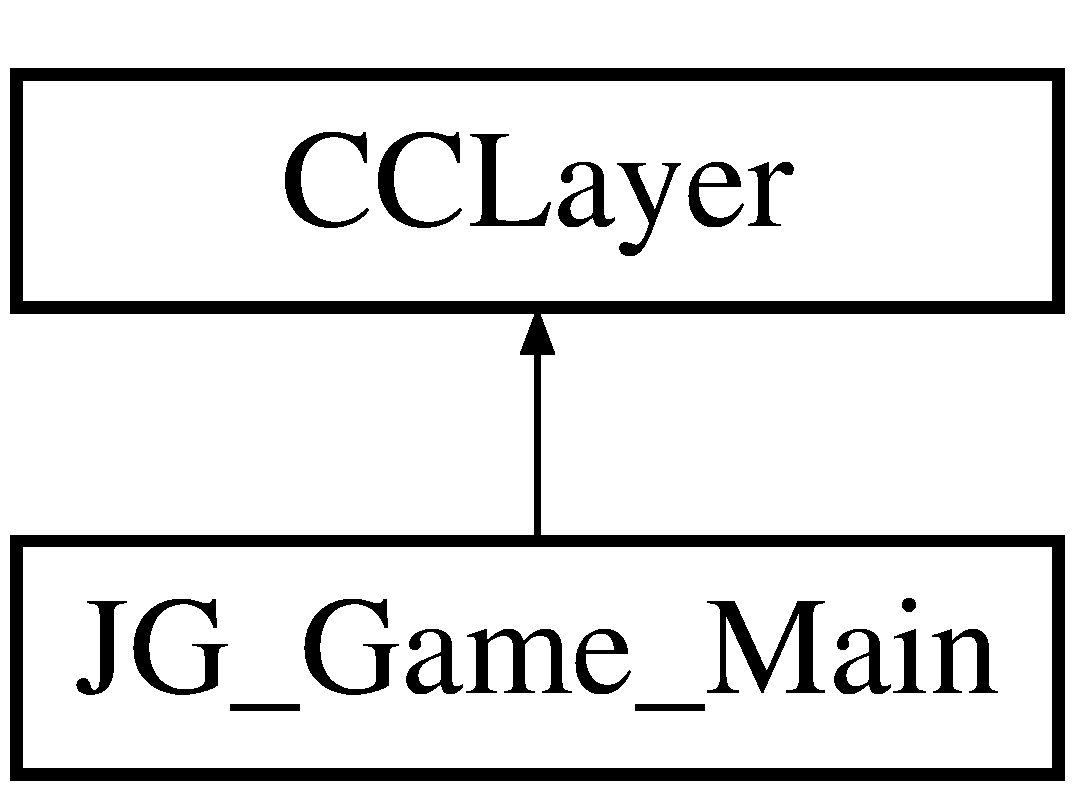
\includegraphics[height=2.000000cm]{class_j_g___game___main}
\end{center}
\end{figure}
\subsection*{Public Member Functions}
\begin{DoxyCompactItemize}
\item 
void \hyperlink{class_j_g___game___main_a36ec5b32f8d745363bafa97dbcfc63fd}{Ball\-Lost} (\hyperlink{class_j_g___ball}{J\-G\-\_\-\-Ball} $\ast$lost\-Ball)
\item 
int \hyperlink{class_j_g___game___main_afa38293cf043c824ccfa4aebe1e1545f}{Get\-Score} ()
\item 
void \hyperlink{class_j_g___game___main_a565135339ab0e993ace77fbfc8b39ab2}{Set\-Score} (int new\-Score)
\item 
void \hyperlink{class_j_g___game___main_af1018c29931a8569a468b0b7495ca5cc}{Add\-Score} (int amount)
\item 
void \hyperlink{class_j_g___game___main_a30a9fb93f7a2a61ce90ab1a77525c006}{Reduce\-Score} (int amount)
\item 
int \hyperlink{class_j_g___game___main_a666b141713d126df7e171fc68dd257a2}{Get\-Life\-Count} ()
\item 
void \hyperlink{class_j_g___game___main_a80e74d397b65b98182fb5c2054632899}{Set\-Life\-Count} (int new\-Life\-Count)
\item 
void \hyperlink{class_j_g___game___main_abffce98f5d7c28791aa13e4d081da6ec}{Decrement\-Life\-Count} ()
\item 
void \hyperlink{class_j_g___game___main_a529a8f577bb296cbbe9143f99ae26f1b}{Increment\-Life\-Count} ()
\item 
\hypertarget{class_j_g___game___main_a4d1e63d731fabbe9e57383254a4b21bf}{virtual bool {\bfseries init} ()}\label{class_j_g___game___main_a4d1e63d731fabbe9e57383254a4b21bf}

\item 
void \hyperlink{class_j_g___game___main_ab7f59e22bd1ddc6f849ceb4731e6f123}{Init\-Game} ()
\item 
virtual void \hyperlink{class_j_g___game___main_a9c8aac91fd97b7a88da7819b8ead4206}{cc\-Touches\-Began} (C\-C\-Set $\ast$p\-Touches, C\-C\-Event $\ast$event)
\item 
virtual void \hyperlink{class_j_g___game___main_ad3ecad4bd190ff37f5b6ba1da9fbe16c}{cc\-Touches\-Moved} (C\-C\-Set $\ast$p\-Touches, C\-C\-Event $\ast$event)
\item 
virtual void \hyperlink{class_j_g___game___main_a0bc1f108b8a56226cfe84ce9d28d56b4}{cc\-Touches\-Ended} (C\-C\-Set $\ast$p\-Touches, C\-C\-Event $\ast$event)
\item 
void \hyperlink{class_j_g___game___main_afe6f0284267c514ca1c81673d015ad91}{Ball\-Touch\-Handler\-\_\-\-Init} (C\-C\-Touch $\ast$touch)
\item 
void \hyperlink{class_j_g___game___main_aa0d9b99e2acd78c8763557d1c0e8a244}{Ball\-Touch\-Handler\-\_\-\-Check\-Direction} (unsigned int index)
\item 
void \hyperlink{class_j_g___game___main_af02d329a7f3a6ac86d8b233dd9ff0741}{Ball\-Touch\-Handler\-\_\-\-End} (unsigned int index)
\item 
void \hyperlink{class_j_g___game___main_a4accf9781acdb8a94450eca925574902}{Ball\-Touch\-Handler\-\_\-\-Check\-Time} (float dt)
\item 
float \hyperlink{class_j_g___game___main_a3b28b2a51aeaa909d6fb95471103bb72}{Calculate\-Throw\-Force} (unsigned int index)
\item 
void \hyperlink{class_j_g___game___main_aea78b9aef2cf228b6945fa88bf741c3a}{update} (float dt)
\item 
bool \hyperlink{class_j_g___game___main_a0b93b253ff5f67b688c12848c63c9e2c}{Are\-Points\-Colliding} (C\-C\-Point point1, C\-C\-Point point2, float radius)
\item 
void \hyperlink{class_j_g___game___main_abda6daf16a4bdfb1d197bcedce380f8e}{Set\-Touch\-Info} (C\-C\-Touch $\ast$touch, \hyperlink{class_j_g___hand}{J\-G\-\_\-\-Hand} $\ast$hand, \hyperlink{class_j_g___ball}{J\-G\-\_\-\-Ball} $\ast$ball)
\item 
void \hyperlink{class_j_g___game___main_a24a120d001b984dc67f211cdb79ce811}{Reset\-Touch\-Info} (int index)
\item 
void \hyperlink{class_j_g___game___main_a2f8dd795fb006e6b052dbe29aef917cf}{Reset\-Touch\-Info\-By\-Ball} (\hyperlink{class_j_g___ball}{J\-G\-\_\-\-Ball} $\ast$ball)
\item 
bool \hyperlink{class_j_g___game___main_a0fab6585f29f1324aea00bdade4e01f4}{Set\-Touch\-Direction\-For\-Ball} (int index)
\item 
\hypertarget{class_j_g___game___main_a42558255c3477748cfadf9d501a02b56}{void {\bfseries menu\-Close\-Callback} (C\-C\-Object $\ast$p\-Sender)}\label{class_j_g___game___main_a42558255c3477748cfadf9d501a02b56}

\item 
\hypertarget{class_j_g___game___main_a2e2740b51a8e5ac7b981078dbd7bbd70}{void {\bfseries menu\-Pause\-Call\-Back} (C\-C\-Object $\ast$p\-Sender)}\label{class_j_g___game___main_a2e2740b51a8e5ac7b981078dbd7bbd70}

\item 
void \hyperlink{class_j_g___game___main_adc1658ea07b4deb55bfe22df04b61aa2}{Remove\-Ball\-From\-Screen} (\hyperlink{class_j_g___ball}{J\-G\-\_\-\-Ball} $\ast$ball)
\item 
void \hyperlink{class_j_g___game___main_a3b5871764fe94896c274e2a072c00dda}{Remove\-All\-Balls\-From\-Screen} ()
\item 
void \hyperlink{class_j_g___game___main_ae827327aa2c6e58cee824a6f5010f5fe}{Add\-Ball\-To\-Screen} ()
\item 
\hypertarget{class_j_g___game___main_aa386bd7cdada1f23b0b32526e67cc2b0}{float {\bfseries get\-Sign} (float num)}\label{class_j_g___game___main_aa386bd7cdada1f23b0b32526e67cc2b0}

\item 
\hypertarget{class_j_g___game___main_ad94a26b81515a717556314a3a8c65b31}{{\bfseries C\-R\-E\-A\-T\-E\-\_\-\-F\-U\-N\-C} (\hyperlink{class_j_g___game___main}{J\-G\-\_\-\-Game\-\_\-\-Main})}\label{class_j_g___game___main_ad94a26b81515a717556314a3a8c65b31}

\item 
void \hyperlink{class_j_g___game___main_ad4691efc615e12254ea347a7b21cd167}{Test\-Single\-Touch} ()
\item 
void \hyperlink{class_j_g___game___main_a5ad7dc858f795f34d33c13b712880b43}{Test\-Multi\-Touch} ()
\item 
void \hyperlink{class_j_g___game___main_a104c8ad94eb551ad2ba292aa46c0298c}{Test\-Multi\-Touch\-\_\-\-Initi\-Touch\-Gen} (float dt=0)
\item 
void \hyperlink{class_j_g___game___main_ae410c7d1cc74a9e7bf6bc51b525f889e}{Test\-Multi\-Touch\-\_\-\-Movement\-Touch\-Gen} (float dt=0)
\item 
void \hyperlink{class_j_g___game___main_ab2d7fb8240de8466d624a2f187d5eadf}{Test\-Multi\-Touch\-\_\-\-End\-Gen} (float dt=0)
\item 
void \hyperlink{class_j_g___game___main_a925a777f7a94c35b278434ff642b623b}{End\-Game} ()
\item 
void \hyperlink{class_j_g___game___main_a511aee5105b667f9d781030e1bdd7d16}{Pause\-Game} (C\-C\-Object $\ast$p\-Sender)
\item 
void \hyperlink{class_j_g___game___main_ad7a6bcb044fcd6f415bf005b8682de9b}{Exit\-Game} (C\-C\-Object $\ast$p\-Sender)
\item 
void \hyperlink{class_j_g___game___main_a0e1494d3e5c8c0a22f0d202716923839}{Resume\-Game} (C\-C\-Object $\ast$p\-Sender)
\item 
void \hyperlink{class_j_g___game___main_a186a53d9b5956462dd186a48adaf251c}{Reset\-Game} (C\-C\-Object $\ast$p\-Sender)
\item 
\hypertarget{class_j_g___game___main_abbbc10c904cdcba09260c925c36d0f22}{void {\bfseries Temp\-Add\-Ball} (float time)}\label{class_j_g___game___main_abbbc10c904cdcba09260c925c36d0f22}

\end{DoxyCompactItemize}
\subsection*{Static Public Member Functions}
\begin{DoxyCompactItemize}
\item 
\hypertarget{class_j_g___game___main_ad8df9f7dc524c5e4096ba72ca3d225a0}{static cocos2d\-::\-C\-C\-Scene $\ast$ {\bfseries scene} ()}\label{class_j_g___game___main_ad8df9f7dc524c5e4096ba72ca3d225a0}

\end{DoxyCompactItemize}
\subsection*{Public Attributes}
\begin{DoxyCompactItemize}
\item 
\hypertarget{class_j_g___game___main_a3312f494aeb62375e2ba54cfc2e7b4f9}{\hyperlink{class_j_g___game___h_u_d}{J\-G\-\_\-\-Game\-\_\-\-H\-U\-D} $\ast$ {\bfseries game\-H\-U\-D}}\label{class_j_g___game___main_a3312f494aeb62375e2ba54cfc2e7b4f9}

\item 
\hypertarget{class_j_g___game___main_a6946a041c2d1e0e1af8f668df4eaef1d}{int {\bfseries life\-Count}}\label{class_j_g___game___main_a6946a041c2d1e0e1af8f668df4eaef1d}

\item 
\hypertarget{class_j_g___game___main_a092aed9f82afd093223436207aaf95ee}{int {\bfseries score}}\label{class_j_g___game___main_a092aed9f82afd093223436207aaf95ee}

\item 
\hypertarget{class_j_g___game___main_a8974bfdd52077060e4561210cabd193f}{C\-C\-Size {\bfseries screen\-Size}}\label{class_j_g___game___main_a8974bfdd52077060e4561210cabd193f}

\item 
C\-C\-Set $\ast$ \hyperlink{class_j_g___game___main_abf4ca18c92688188dcf7bf60c73fa3ae}{Test\-Multi\-Touches\-Set}
\end{DoxyCompactItemize}


\subsection{Detailed Description}
The main class for controlling the game 

\subsection{Member Function Documentation}
\hypertarget{class_j_g___game___main_ae827327aa2c6e58cee824a6f5010f5fe}{\index{J\-G\-\_\-\-Game\-\_\-\-Main@{J\-G\-\_\-\-Game\-\_\-\-Main}!Add\-Ball\-To\-Screen@{Add\-Ball\-To\-Screen}}
\index{Add\-Ball\-To\-Screen@{Add\-Ball\-To\-Screen}!JG_Game_Main@{J\-G\-\_\-\-Game\-\_\-\-Main}}
\subsubsection[{Add\-Ball\-To\-Screen}]{\setlength{\rightskip}{0pt plus 5cm}void J\-G\-\_\-\-Game\-\_\-\-Main\-::\-Add\-Ball\-To\-Screen (
\begin{DoxyParamCaption}
{}
\end{DoxyParamCaption}
)}}\label{class_j_g___game___main_ae827327aa2c6e58cee824a6f5010f5fe}
Adding new ball to screen \hypertarget{class_j_g___game___main_af1018c29931a8569a468b0b7495ca5cc}{\index{J\-G\-\_\-\-Game\-\_\-\-Main@{J\-G\-\_\-\-Game\-\_\-\-Main}!Add\-Score@{Add\-Score}}
\index{Add\-Score@{Add\-Score}!JG_Game_Main@{J\-G\-\_\-\-Game\-\_\-\-Main}}
\subsubsection[{Add\-Score}]{\setlength{\rightskip}{0pt plus 5cm}void J\-G\-\_\-\-Game\-\_\-\-Main\-::\-Add\-Score (
\begin{DoxyParamCaption}
\item[{int}]{amount}
\end{DoxyParamCaption}
)}}\label{class_j_g___game___main_af1018c29931a8569a468b0b7495ca5cc}
Add a value to player score \hypertarget{class_j_g___game___main_a0b93b253ff5f67b688c12848c63c9e2c}{\index{J\-G\-\_\-\-Game\-\_\-\-Main@{J\-G\-\_\-\-Game\-\_\-\-Main}!Are\-Points\-Colliding@{Are\-Points\-Colliding}}
\index{Are\-Points\-Colliding@{Are\-Points\-Colliding}!JG_Game_Main@{J\-G\-\_\-\-Game\-\_\-\-Main}}
\subsubsection[{Are\-Points\-Colliding}]{\setlength{\rightskip}{0pt plus 5cm}bool J\-G\-\_\-\-Game\-\_\-\-Main\-::\-Are\-Points\-Colliding (
\begin{DoxyParamCaption}
\item[{C\-C\-Point}]{point1, }
\item[{C\-C\-Point}]{point2, }
\item[{float}]{radius}
\end{DoxyParamCaption}
)}}\label{class_j_g___game___main_a0b93b253ff5f67b688c12848c63c9e2c}
checks whether distance of the two point are lesser than radius or not \hypertarget{class_j_g___game___main_a36ec5b32f8d745363bafa97dbcfc63fd}{\index{J\-G\-\_\-\-Game\-\_\-\-Main@{J\-G\-\_\-\-Game\-\_\-\-Main}!Ball\-Lost@{Ball\-Lost}}
\index{Ball\-Lost@{Ball\-Lost}!JG_Game_Main@{J\-G\-\_\-\-Game\-\_\-\-Main}}
\subsubsection[{Ball\-Lost}]{\setlength{\rightskip}{0pt plus 5cm}void J\-G\-\_\-\-Game\-\_\-\-Main\-::\-Ball\-Lost (
\begin{DoxyParamCaption}
\item[{{\bf J\-G\-\_\-\-Ball} $\ast$}]{lost\-Ball}
\end{DoxyParamCaption}
)}}\label{class_j_g___game___main_a36ec5b32f8d745363bafa97dbcfc63fd}
this method is called when a ball is lost ( for now when it is out of screen ) \hypertarget{class_j_g___game___main_aa0d9b99e2acd78c8763557d1c0e8a244}{\index{J\-G\-\_\-\-Game\-\_\-\-Main@{J\-G\-\_\-\-Game\-\_\-\-Main}!Ball\-Touch\-Handler\-\_\-\-Check\-Direction@{Ball\-Touch\-Handler\-\_\-\-Check\-Direction}}
\index{Ball\-Touch\-Handler\-\_\-\-Check\-Direction@{Ball\-Touch\-Handler\-\_\-\-Check\-Direction}!JG_Game_Main@{J\-G\-\_\-\-Game\-\_\-\-Main}}
\subsubsection[{Ball\-Touch\-Handler\-\_\-\-Check\-Direction}]{\setlength{\rightskip}{0pt plus 5cm}void J\-G\-\_\-\-Game\-\_\-\-Main\-::\-Ball\-Touch\-Handler\-\_\-\-Check\-Direction (
\begin{DoxyParamCaption}
\item[{unsigned int}]{index}
\end{DoxyParamCaption}
)}}\label{class_j_g___game___main_aa0d9b99e2acd78c8763557d1c0e8a244}
check direction of the ball \hypertarget{class_j_g___game___main_a4accf9781acdb8a94450eca925574902}{\index{J\-G\-\_\-\-Game\-\_\-\-Main@{J\-G\-\_\-\-Game\-\_\-\-Main}!Ball\-Touch\-Handler\-\_\-\-Check\-Time@{Ball\-Touch\-Handler\-\_\-\-Check\-Time}}
\index{Ball\-Touch\-Handler\-\_\-\-Check\-Time@{Ball\-Touch\-Handler\-\_\-\-Check\-Time}!JG_Game_Main@{J\-G\-\_\-\-Game\-\_\-\-Main}}
\subsubsection[{Ball\-Touch\-Handler\-\_\-\-Check\-Time}]{\setlength{\rightskip}{0pt plus 5cm}void J\-G\-\_\-\-Game\-\_\-\-Main\-::\-Ball\-Touch\-Handler\-\_\-\-Check\-Time (
\begin{DoxyParamCaption}
\item[{float}]{dt}
\end{DoxyParamCaption}
)}}\label{class_j_g___game___main_a4accf9781acdb8a94450eca925574902}
it handle the time player hold his touch on the screen \hypertarget{class_j_g___game___main_af02d329a7f3a6ac86d8b233dd9ff0741}{\index{J\-G\-\_\-\-Game\-\_\-\-Main@{J\-G\-\_\-\-Game\-\_\-\-Main}!Ball\-Touch\-Handler\-\_\-\-End@{Ball\-Touch\-Handler\-\_\-\-End}}
\index{Ball\-Touch\-Handler\-\_\-\-End@{Ball\-Touch\-Handler\-\_\-\-End}!JG_Game_Main@{J\-G\-\_\-\-Game\-\_\-\-Main}}
\subsubsection[{Ball\-Touch\-Handler\-\_\-\-End}]{\setlength{\rightskip}{0pt plus 5cm}void J\-G\-\_\-\-Game\-\_\-\-Main\-::\-Ball\-Touch\-Handler\-\_\-\-End (
\begin{DoxyParamCaption}
\item[{unsigned int}]{index}
\end{DoxyParamCaption}
)}}\label{class_j_g___game___main_af02d329a7f3a6ac86d8b233dd9ff0741}
handling the throwing of the ball \hypertarget{class_j_g___game___main_afe6f0284267c514ca1c81673d015ad91}{\index{J\-G\-\_\-\-Game\-\_\-\-Main@{J\-G\-\_\-\-Game\-\_\-\-Main}!Ball\-Touch\-Handler\-\_\-\-Init@{Ball\-Touch\-Handler\-\_\-\-Init}}
\index{Ball\-Touch\-Handler\-\_\-\-Init@{Ball\-Touch\-Handler\-\_\-\-Init}!JG_Game_Main@{J\-G\-\_\-\-Game\-\_\-\-Main}}
\subsubsection[{Ball\-Touch\-Handler\-\_\-\-Init}]{\setlength{\rightskip}{0pt plus 5cm}void J\-G\-\_\-\-Game\-\_\-\-Main\-::\-Ball\-Touch\-Handler\-\_\-\-Init (
\begin{DoxyParamCaption}
\item[{C\-C\-Touch $\ast$}]{touch}
\end{DoxyParamCaption}
)}}\label{class_j_g___game___main_afe6f0284267c514ca1c81673d015ad91}
defined to handle initiation of touch \hypertarget{class_j_g___game___main_a3b28b2a51aeaa909d6fb95471103bb72}{\index{J\-G\-\_\-\-Game\-\_\-\-Main@{J\-G\-\_\-\-Game\-\_\-\-Main}!Calculate\-Throw\-Force@{Calculate\-Throw\-Force}}
\index{Calculate\-Throw\-Force@{Calculate\-Throw\-Force}!JG_Game_Main@{J\-G\-\_\-\-Game\-\_\-\-Main}}
\subsubsection[{Calculate\-Throw\-Force}]{\setlength{\rightskip}{0pt plus 5cm}float J\-G\-\_\-\-Game\-\_\-\-Main\-::\-Calculate\-Throw\-Force (
\begin{DoxyParamCaption}
\item[{unsigned int}]{index}
\end{DoxyParamCaption}
)}}\label{class_j_g___game___main_a3b28b2a51aeaa909d6fb95471103bb72}
to calculate the force of the touch \hypertarget{class_j_g___game___main_a9c8aac91fd97b7a88da7819b8ead4206}{\index{J\-G\-\_\-\-Game\-\_\-\-Main@{J\-G\-\_\-\-Game\-\_\-\-Main}!cc\-Touches\-Began@{cc\-Touches\-Began}}
\index{cc\-Touches\-Began@{cc\-Touches\-Began}!JG_Game_Main@{J\-G\-\_\-\-Game\-\_\-\-Main}}
\subsubsection[{cc\-Touches\-Began}]{\setlength{\rightskip}{0pt plus 5cm}void J\-G\-\_\-\-Game\-\_\-\-Main\-::cc\-Touches\-Began (
\begin{DoxyParamCaption}
\item[{C\-C\-Set $\ast$}]{p\-Touches, }
\item[{C\-C\-Event $\ast$}]{event}
\end{DoxyParamCaption}
)\hspace{0.3cm}{\ttfamily [virtual]}}}\label{class_j_g___game___main_a9c8aac91fd97b7a88da7819b8ead4206}
Handles the beginning of the touch \hypertarget{class_j_g___game___main_a0bc1f108b8a56226cfe84ce9d28d56b4}{\index{J\-G\-\_\-\-Game\-\_\-\-Main@{J\-G\-\_\-\-Game\-\_\-\-Main}!cc\-Touches\-Ended@{cc\-Touches\-Ended}}
\index{cc\-Touches\-Ended@{cc\-Touches\-Ended}!JG_Game_Main@{J\-G\-\_\-\-Game\-\_\-\-Main}}
\subsubsection[{cc\-Touches\-Ended}]{\setlength{\rightskip}{0pt plus 5cm}void J\-G\-\_\-\-Game\-\_\-\-Main\-::cc\-Touches\-Ended (
\begin{DoxyParamCaption}
\item[{C\-C\-Set $\ast$}]{p\-Touches, }
\item[{C\-C\-Event $\ast$}]{event}
\end{DoxyParamCaption}
)\hspace{0.3cm}{\ttfamily [virtual]}}}\label{class_j_g___game___main_a0bc1f108b8a56226cfe84ce9d28d56b4}
Handles the end of the touch \hypertarget{class_j_g___game___main_ad3ecad4bd190ff37f5b6ba1da9fbe16c}{\index{J\-G\-\_\-\-Game\-\_\-\-Main@{J\-G\-\_\-\-Game\-\_\-\-Main}!cc\-Touches\-Moved@{cc\-Touches\-Moved}}
\index{cc\-Touches\-Moved@{cc\-Touches\-Moved}!JG_Game_Main@{J\-G\-\_\-\-Game\-\_\-\-Main}}
\subsubsection[{cc\-Touches\-Moved}]{\setlength{\rightskip}{0pt plus 5cm}void J\-G\-\_\-\-Game\-\_\-\-Main\-::cc\-Touches\-Moved (
\begin{DoxyParamCaption}
\item[{C\-C\-Set $\ast$}]{p\-Touches, }
\item[{C\-C\-Event $\ast$}]{event}
\end{DoxyParamCaption}
)\hspace{0.3cm}{\ttfamily [virtual]}}}\label{class_j_g___game___main_ad3ecad4bd190ff37f5b6ba1da9fbe16c}
Handles the movement of the touch \hypertarget{class_j_g___game___main_abffce98f5d7c28791aa13e4d081da6ec}{\index{J\-G\-\_\-\-Game\-\_\-\-Main@{J\-G\-\_\-\-Game\-\_\-\-Main}!Decrement\-Life\-Count@{Decrement\-Life\-Count}}
\index{Decrement\-Life\-Count@{Decrement\-Life\-Count}!JG_Game_Main@{J\-G\-\_\-\-Game\-\_\-\-Main}}
\subsubsection[{Decrement\-Life\-Count}]{\setlength{\rightskip}{0pt plus 5cm}void J\-G\-\_\-\-Game\-\_\-\-Main\-::\-Decrement\-Life\-Count (
\begin{DoxyParamCaption}
{}
\end{DoxyParamCaption}
)}}\label{class_j_g___game___main_abffce98f5d7c28791aa13e4d081da6ec}
Decrement the life count of player \hypertarget{class_j_g___game___main_a925a777f7a94c35b278434ff642b623b}{\index{J\-G\-\_\-\-Game\-\_\-\-Main@{J\-G\-\_\-\-Game\-\_\-\-Main}!End\-Game@{End\-Game}}
\index{End\-Game@{End\-Game}!JG_Game_Main@{J\-G\-\_\-\-Game\-\_\-\-Main}}
\subsubsection[{End\-Game}]{\setlength{\rightskip}{0pt plus 5cm}void J\-G\-\_\-\-Game\-\_\-\-Main\-::\-End\-Game (
\begin{DoxyParamCaption}
{}
\end{DoxyParamCaption}
)}}\label{class_j_g___game___main_a925a777f7a94c35b278434ff642b623b}
End of the game \hypertarget{class_j_g___game___main_ad7a6bcb044fcd6f415bf005b8682de9b}{\index{J\-G\-\_\-\-Game\-\_\-\-Main@{J\-G\-\_\-\-Game\-\_\-\-Main}!Exit\-Game@{Exit\-Game}}
\index{Exit\-Game@{Exit\-Game}!JG_Game_Main@{J\-G\-\_\-\-Game\-\_\-\-Main}}
\subsubsection[{Exit\-Game}]{\setlength{\rightskip}{0pt plus 5cm}void J\-G\-\_\-\-Game\-\_\-\-Main\-::\-Exit\-Game (
\begin{DoxyParamCaption}
\item[{C\-C\-Object $\ast$}]{p\-Sender}
\end{DoxyParamCaption}
)}}\label{class_j_g___game___main_ad7a6bcb044fcd6f415bf005b8682de9b}
Exit the game \hypertarget{class_j_g___game___main_a666b141713d126df7e171fc68dd257a2}{\index{J\-G\-\_\-\-Game\-\_\-\-Main@{J\-G\-\_\-\-Game\-\_\-\-Main}!Get\-Life\-Count@{Get\-Life\-Count}}
\index{Get\-Life\-Count@{Get\-Life\-Count}!JG_Game_Main@{J\-G\-\_\-\-Game\-\_\-\-Main}}
\subsubsection[{Get\-Life\-Count}]{\setlength{\rightskip}{0pt plus 5cm}int J\-G\-\_\-\-Game\-\_\-\-Main\-::\-Get\-Life\-Count (
\begin{DoxyParamCaption}
{}
\end{DoxyParamCaption}
)}}\label{class_j_g___game___main_a666b141713d126df7e171fc68dd257a2}
Return The life count of player \hypertarget{class_j_g___game___main_afa38293cf043c824ccfa4aebe1e1545f}{\index{J\-G\-\_\-\-Game\-\_\-\-Main@{J\-G\-\_\-\-Game\-\_\-\-Main}!Get\-Score@{Get\-Score}}
\index{Get\-Score@{Get\-Score}!JG_Game_Main@{J\-G\-\_\-\-Game\-\_\-\-Main}}
\subsubsection[{Get\-Score}]{\setlength{\rightskip}{0pt plus 5cm}int J\-G\-\_\-\-Game\-\_\-\-Main\-::\-Get\-Score (
\begin{DoxyParamCaption}
{}
\end{DoxyParamCaption}
)}}\label{class_j_g___game___main_afa38293cf043c824ccfa4aebe1e1545f}
Return player Score \hypertarget{class_j_g___game___main_a529a8f577bb296cbbe9143f99ae26f1b}{\index{J\-G\-\_\-\-Game\-\_\-\-Main@{J\-G\-\_\-\-Game\-\_\-\-Main}!Increment\-Life\-Count@{Increment\-Life\-Count}}
\index{Increment\-Life\-Count@{Increment\-Life\-Count}!JG_Game_Main@{J\-G\-\_\-\-Game\-\_\-\-Main}}
\subsubsection[{Increment\-Life\-Count}]{\setlength{\rightskip}{0pt plus 5cm}void J\-G\-\_\-\-Game\-\_\-\-Main\-::\-Increment\-Life\-Count (
\begin{DoxyParamCaption}
{}
\end{DoxyParamCaption}
)}}\label{class_j_g___game___main_a529a8f577bb296cbbe9143f99ae26f1b}
Increment the life count of player \hypertarget{class_j_g___game___main_ab7f59e22bd1ddc6f849ceb4731e6f123}{\index{J\-G\-\_\-\-Game\-\_\-\-Main@{J\-G\-\_\-\-Game\-\_\-\-Main}!Init\-Game@{Init\-Game}}
\index{Init\-Game@{Init\-Game}!JG_Game_Main@{J\-G\-\_\-\-Game\-\_\-\-Main}}
\subsubsection[{Init\-Game}]{\setlength{\rightskip}{0pt plus 5cm}void J\-G\-\_\-\-Game\-\_\-\-Main\-::\-Init\-Game (
\begin{DoxyParamCaption}
{}
\end{DoxyParamCaption}
)}}\label{class_j_g___game___main_ab7f59e22bd1ddc6f849ceb4731e6f123}
Initial the game state \hypertarget{class_j_g___game___main_a511aee5105b667f9d781030e1bdd7d16}{\index{J\-G\-\_\-\-Game\-\_\-\-Main@{J\-G\-\_\-\-Game\-\_\-\-Main}!Pause\-Game@{Pause\-Game}}
\index{Pause\-Game@{Pause\-Game}!JG_Game_Main@{J\-G\-\_\-\-Game\-\_\-\-Main}}
\subsubsection[{Pause\-Game}]{\setlength{\rightskip}{0pt plus 5cm}void J\-G\-\_\-\-Game\-\_\-\-Main\-::\-Pause\-Game (
\begin{DoxyParamCaption}
\item[{C\-C\-Object $\ast$}]{p\-Sender}
\end{DoxyParamCaption}
)}}\label{class_j_g___game___main_a511aee5105b667f9d781030e1bdd7d16}
Pausing the game \hypertarget{class_j_g___game___main_a30a9fb93f7a2a61ce90ab1a77525c006}{\index{J\-G\-\_\-\-Game\-\_\-\-Main@{J\-G\-\_\-\-Game\-\_\-\-Main}!Reduce\-Score@{Reduce\-Score}}
\index{Reduce\-Score@{Reduce\-Score}!JG_Game_Main@{J\-G\-\_\-\-Game\-\_\-\-Main}}
\subsubsection[{Reduce\-Score}]{\setlength{\rightskip}{0pt plus 5cm}void J\-G\-\_\-\-Game\-\_\-\-Main\-::\-Reduce\-Score (
\begin{DoxyParamCaption}
\item[{int}]{amount}
\end{DoxyParamCaption}
)}}\label{class_j_g___game___main_a30a9fb93f7a2a61ce90ab1a77525c006}
Reduce a value from player Score \hypertarget{class_j_g___game___main_a3b5871764fe94896c274e2a072c00dda}{\index{J\-G\-\_\-\-Game\-\_\-\-Main@{J\-G\-\_\-\-Game\-\_\-\-Main}!Remove\-All\-Balls\-From\-Screen@{Remove\-All\-Balls\-From\-Screen}}
\index{Remove\-All\-Balls\-From\-Screen@{Remove\-All\-Balls\-From\-Screen}!JG_Game_Main@{J\-G\-\_\-\-Game\-\_\-\-Main}}
\subsubsection[{Remove\-All\-Balls\-From\-Screen}]{\setlength{\rightskip}{0pt plus 5cm}void J\-G\-\_\-\-Game\-\_\-\-Main\-::\-Remove\-All\-Balls\-From\-Screen (
\begin{DoxyParamCaption}
{}
\end{DoxyParamCaption}
)}}\label{class_j_g___game___main_a3b5871764fe94896c274e2a072c00dda}
Remove all balls from screen \hypertarget{class_j_g___game___main_adc1658ea07b4deb55bfe22df04b61aa2}{\index{J\-G\-\_\-\-Game\-\_\-\-Main@{J\-G\-\_\-\-Game\-\_\-\-Main}!Remove\-Ball\-From\-Screen@{Remove\-Ball\-From\-Screen}}
\index{Remove\-Ball\-From\-Screen@{Remove\-Ball\-From\-Screen}!JG_Game_Main@{J\-G\-\_\-\-Game\-\_\-\-Main}}
\subsubsection[{Remove\-Ball\-From\-Screen}]{\setlength{\rightskip}{0pt plus 5cm}void J\-G\-\_\-\-Game\-\_\-\-Main\-::\-Remove\-Ball\-From\-Screen (
\begin{DoxyParamCaption}
\item[{{\bf J\-G\-\_\-\-Ball} $\ast$}]{ball}
\end{DoxyParamCaption}
)}}\label{class_j_g___game___main_adc1658ea07b4deb55bfe22df04b61aa2}
handles ball removing \hypertarget{class_j_g___game___main_a186a53d9b5956462dd186a48adaf251c}{\index{J\-G\-\_\-\-Game\-\_\-\-Main@{J\-G\-\_\-\-Game\-\_\-\-Main}!Reset\-Game@{Reset\-Game}}
\index{Reset\-Game@{Reset\-Game}!JG_Game_Main@{J\-G\-\_\-\-Game\-\_\-\-Main}}
\subsubsection[{Reset\-Game}]{\setlength{\rightskip}{0pt plus 5cm}void J\-G\-\_\-\-Game\-\_\-\-Main\-::\-Reset\-Game (
\begin{DoxyParamCaption}
\item[{C\-C\-Object $\ast$}]{p\-Sender}
\end{DoxyParamCaption}
)}}\label{class_j_g___game___main_a186a53d9b5956462dd186a48adaf251c}
Reseting the game \hypertarget{class_j_g___game___main_a24a120d001b984dc67f211cdb79ce811}{\index{J\-G\-\_\-\-Game\-\_\-\-Main@{J\-G\-\_\-\-Game\-\_\-\-Main}!Reset\-Touch\-Info@{Reset\-Touch\-Info}}
\index{Reset\-Touch\-Info@{Reset\-Touch\-Info}!JG_Game_Main@{J\-G\-\_\-\-Game\-\_\-\-Main}}
\subsubsection[{Reset\-Touch\-Info}]{\setlength{\rightskip}{0pt plus 5cm}void J\-G\-\_\-\-Game\-\_\-\-Main\-::\-Reset\-Touch\-Info (
\begin{DoxyParamCaption}
\item[{int}]{index}
\end{DoxyParamCaption}
)}}\label{class_j_g___game___main_a24a120d001b984dc67f211cdb79ce811}
Reset an touchinfo with the given index in touch\-Infos \hypertarget{class_j_g___game___main_a2f8dd795fb006e6b052dbe29aef917cf}{\index{J\-G\-\_\-\-Game\-\_\-\-Main@{J\-G\-\_\-\-Game\-\_\-\-Main}!Reset\-Touch\-Info\-By\-Ball@{Reset\-Touch\-Info\-By\-Ball}}
\index{Reset\-Touch\-Info\-By\-Ball@{Reset\-Touch\-Info\-By\-Ball}!JG_Game_Main@{J\-G\-\_\-\-Game\-\_\-\-Main}}
\subsubsection[{Reset\-Touch\-Info\-By\-Ball}]{\setlength{\rightskip}{0pt plus 5cm}void J\-G\-\_\-\-Game\-\_\-\-Main\-::\-Reset\-Touch\-Info\-By\-Ball (
\begin{DoxyParamCaption}
\item[{{\bf J\-G\-\_\-\-Ball} $\ast$}]{ball}
\end{DoxyParamCaption}
)}}\label{class_j_g___game___main_a2f8dd795fb006e6b052dbe29aef917cf}
Reset an touchinfo with the given ball in touch\-Infos \hypertarget{class_j_g___game___main_a0e1494d3e5c8c0a22f0d202716923839}{\index{J\-G\-\_\-\-Game\-\_\-\-Main@{J\-G\-\_\-\-Game\-\_\-\-Main}!Resume\-Game@{Resume\-Game}}
\index{Resume\-Game@{Resume\-Game}!JG_Game_Main@{J\-G\-\_\-\-Game\-\_\-\-Main}}
\subsubsection[{Resume\-Game}]{\setlength{\rightskip}{0pt plus 5cm}void J\-G\-\_\-\-Game\-\_\-\-Main\-::\-Resume\-Game (
\begin{DoxyParamCaption}
\item[{C\-C\-Object $\ast$}]{p\-Sender}
\end{DoxyParamCaption}
)}}\label{class_j_g___game___main_a0e1494d3e5c8c0a22f0d202716923839}
Resuming the game \hypertarget{class_j_g___game___main_a80e74d397b65b98182fb5c2054632899}{\index{J\-G\-\_\-\-Game\-\_\-\-Main@{J\-G\-\_\-\-Game\-\_\-\-Main}!Set\-Life\-Count@{Set\-Life\-Count}}
\index{Set\-Life\-Count@{Set\-Life\-Count}!JG_Game_Main@{J\-G\-\_\-\-Game\-\_\-\-Main}}
\subsubsection[{Set\-Life\-Count}]{\setlength{\rightskip}{0pt plus 5cm}void J\-G\-\_\-\-Game\-\_\-\-Main\-::\-Set\-Life\-Count (
\begin{DoxyParamCaption}
\item[{int}]{new\-Life\-Count}
\end{DoxyParamCaption}
)}}\label{class_j_g___game___main_a80e74d397b65b98182fb5c2054632899}
Set the life count of player \hypertarget{class_j_g___game___main_a565135339ab0e993ace77fbfc8b39ab2}{\index{J\-G\-\_\-\-Game\-\_\-\-Main@{J\-G\-\_\-\-Game\-\_\-\-Main}!Set\-Score@{Set\-Score}}
\index{Set\-Score@{Set\-Score}!JG_Game_Main@{J\-G\-\_\-\-Game\-\_\-\-Main}}
\subsubsection[{Set\-Score}]{\setlength{\rightskip}{0pt plus 5cm}void J\-G\-\_\-\-Game\-\_\-\-Main\-::\-Set\-Score (
\begin{DoxyParamCaption}
\item[{int}]{new\-Score}
\end{DoxyParamCaption}
)}}\label{class_j_g___game___main_a565135339ab0e993ace77fbfc8b39ab2}
Set player Score to a new value \hypertarget{class_j_g___game___main_a0fab6585f29f1324aea00bdade4e01f4}{\index{J\-G\-\_\-\-Game\-\_\-\-Main@{J\-G\-\_\-\-Game\-\_\-\-Main}!Set\-Touch\-Direction\-For\-Ball@{Set\-Touch\-Direction\-For\-Ball}}
\index{Set\-Touch\-Direction\-For\-Ball@{Set\-Touch\-Direction\-For\-Ball}!JG_Game_Main@{J\-G\-\_\-\-Game\-\_\-\-Main}}
\subsubsection[{Set\-Touch\-Direction\-For\-Ball}]{\setlength{\rightskip}{0pt plus 5cm}bool J\-G\-\_\-\-Game\-\_\-\-Main\-::\-Set\-Touch\-Direction\-For\-Ball (
\begin{DoxyParamCaption}
\item[{int}]{index}
\end{DoxyParamCaption}
)}}\label{class_j_g___game___main_a0fab6585f29f1324aea00bdade4e01f4}
Set Direction For Ball for the give index in touch\-Infos. return whether direction was valid or not \hypertarget{class_j_g___game___main_abda6daf16a4bdfb1d197bcedce380f8e}{\index{J\-G\-\_\-\-Game\-\_\-\-Main@{J\-G\-\_\-\-Game\-\_\-\-Main}!Set\-Touch\-Info@{Set\-Touch\-Info}}
\index{Set\-Touch\-Info@{Set\-Touch\-Info}!JG_Game_Main@{J\-G\-\_\-\-Game\-\_\-\-Main}}
\subsubsection[{Set\-Touch\-Info}]{\setlength{\rightskip}{0pt plus 5cm}void J\-G\-\_\-\-Game\-\_\-\-Main\-::\-Set\-Touch\-Info (
\begin{DoxyParamCaption}
\item[{C\-C\-Touch $\ast$}]{touch, }
\item[{{\bf J\-G\-\_\-\-Hand} $\ast$}]{hand, }
\item[{{\bf J\-G\-\_\-\-Ball} $\ast$}]{ball}
\end{DoxyParamCaption}
)}}\label{class_j_g___game___main_abda6daf16a4bdfb1d197bcedce380f8e}
Set an empty touchinfo with a new info \hypertarget{class_j_g___game___main_a5ad7dc858f795f34d33c13b712880b43}{\index{J\-G\-\_\-\-Game\-\_\-\-Main@{J\-G\-\_\-\-Game\-\_\-\-Main}!Test\-Multi\-Touch@{Test\-Multi\-Touch}}
\index{Test\-Multi\-Touch@{Test\-Multi\-Touch}!JG_Game_Main@{J\-G\-\_\-\-Game\-\_\-\-Main}}
\subsubsection[{Test\-Multi\-Touch}]{\setlength{\rightskip}{0pt plus 5cm}void J\-G\-\_\-\-Game\-\_\-\-Main\-::\-Test\-Multi\-Touch (
\begin{DoxyParamCaption}
{}
\end{DoxyParamCaption}
)}}\label{class_j_g___game___main_a5ad7dc858f795f34d33c13b712880b43}
Testing Multi\-Touch Handling \hypertarget{class_j_g___game___main_ab2d7fb8240de8466d624a2f187d5eadf}{\index{J\-G\-\_\-\-Game\-\_\-\-Main@{J\-G\-\_\-\-Game\-\_\-\-Main}!Test\-Multi\-Touch\-\_\-\-End\-Gen@{Test\-Multi\-Touch\-\_\-\-End\-Gen}}
\index{Test\-Multi\-Touch\-\_\-\-End\-Gen@{Test\-Multi\-Touch\-\_\-\-End\-Gen}!JG_Game_Main@{J\-G\-\_\-\-Game\-\_\-\-Main}}
\subsubsection[{Test\-Multi\-Touch\-\_\-\-End\-Gen}]{\setlength{\rightskip}{0pt plus 5cm}void J\-G\-\_\-\-Game\-\_\-\-Main\-::\-Test\-Multi\-Touch\-\_\-\-End\-Gen (
\begin{DoxyParamCaption}
\item[{float}]{dt = {\ttfamily 0}}
\end{DoxyParamCaption}
)}}\label{class_j_g___game___main_ab2d7fb8240de8466d624a2f187d5eadf}
End phase of multi touch testing \hypertarget{class_j_g___game___main_a104c8ad94eb551ad2ba292aa46c0298c}{\index{J\-G\-\_\-\-Game\-\_\-\-Main@{J\-G\-\_\-\-Game\-\_\-\-Main}!Test\-Multi\-Touch\-\_\-\-Initi\-Touch\-Gen@{Test\-Multi\-Touch\-\_\-\-Initi\-Touch\-Gen}}
\index{Test\-Multi\-Touch\-\_\-\-Initi\-Touch\-Gen@{Test\-Multi\-Touch\-\_\-\-Initi\-Touch\-Gen}!JG_Game_Main@{J\-G\-\_\-\-Game\-\_\-\-Main}}
\subsubsection[{Test\-Multi\-Touch\-\_\-\-Initi\-Touch\-Gen}]{\setlength{\rightskip}{0pt plus 5cm}void J\-G\-\_\-\-Game\-\_\-\-Main\-::\-Test\-Multi\-Touch\-\_\-\-Initi\-Touch\-Gen (
\begin{DoxyParamCaption}
\item[{float}]{dt = {\ttfamily 0}}
\end{DoxyParamCaption}
)}}\label{class_j_g___game___main_a104c8ad94eb551ad2ba292aa46c0298c}
Initial phase of multi touch testing \hypertarget{class_j_g___game___main_ae410c7d1cc74a9e7bf6bc51b525f889e}{\index{J\-G\-\_\-\-Game\-\_\-\-Main@{J\-G\-\_\-\-Game\-\_\-\-Main}!Test\-Multi\-Touch\-\_\-\-Movement\-Touch\-Gen@{Test\-Multi\-Touch\-\_\-\-Movement\-Touch\-Gen}}
\index{Test\-Multi\-Touch\-\_\-\-Movement\-Touch\-Gen@{Test\-Multi\-Touch\-\_\-\-Movement\-Touch\-Gen}!JG_Game_Main@{J\-G\-\_\-\-Game\-\_\-\-Main}}
\subsubsection[{Test\-Multi\-Touch\-\_\-\-Movement\-Touch\-Gen}]{\setlength{\rightskip}{0pt plus 5cm}void J\-G\-\_\-\-Game\-\_\-\-Main\-::\-Test\-Multi\-Touch\-\_\-\-Movement\-Touch\-Gen (
\begin{DoxyParamCaption}
\item[{float}]{dt = {\ttfamily 0}}
\end{DoxyParamCaption}
)}}\label{class_j_g___game___main_ae410c7d1cc74a9e7bf6bc51b525f889e}
Movement phase of multi touch testing \hypertarget{class_j_g___game___main_ad4691efc615e12254ea347a7b21cd167}{\index{J\-G\-\_\-\-Game\-\_\-\-Main@{J\-G\-\_\-\-Game\-\_\-\-Main}!Test\-Single\-Touch@{Test\-Single\-Touch}}
\index{Test\-Single\-Touch@{Test\-Single\-Touch}!JG_Game_Main@{J\-G\-\_\-\-Game\-\_\-\-Main}}
\subsubsection[{Test\-Single\-Touch}]{\setlength{\rightskip}{0pt plus 5cm}void J\-G\-\_\-\-Game\-\_\-\-Main\-::\-Test\-Single\-Touch (
\begin{DoxyParamCaption}
{}
\end{DoxyParamCaption}
)}}\label{class_j_g___game___main_ad4691efc615e12254ea347a7b21cd167}
a function to test single touch \hypertarget{class_j_g___game___main_aea78b9aef2cf228b6945fa88bf741c3a}{\index{J\-G\-\_\-\-Game\-\_\-\-Main@{J\-G\-\_\-\-Game\-\_\-\-Main}!update@{update}}
\index{update@{update}!JG_Game_Main@{J\-G\-\_\-\-Game\-\_\-\-Main}}
\subsubsection[{update}]{\setlength{\rightskip}{0pt plus 5cm}void J\-G\-\_\-\-Game\-\_\-\-Main\-::update (
\begin{DoxyParamCaption}
\item[{float}]{dt}
\end{DoxyParamCaption}
)}}\label{class_j_g___game___main_aea78b9aef2cf228b6945fa88bf741c3a}
update function 

\subsection{Member Data Documentation}
\hypertarget{class_j_g___game___main_abf4ca18c92688188dcf7bf60c73fa3ae}{\index{J\-G\-\_\-\-Game\-\_\-\-Main@{J\-G\-\_\-\-Game\-\_\-\-Main}!Test\-Multi\-Touches\-Set@{Test\-Multi\-Touches\-Set}}
\index{Test\-Multi\-Touches\-Set@{Test\-Multi\-Touches\-Set}!JG_Game_Main@{J\-G\-\_\-\-Game\-\_\-\-Main}}
\subsubsection[{Test\-Multi\-Touches\-Set}]{\setlength{\rightskip}{0pt plus 5cm}C\-C\-Set$\ast$ J\-G\-\_\-\-Game\-\_\-\-Main\-::\-Test\-Multi\-Touches\-Set}}\label{class_j_g___game___main_abf4ca18c92688188dcf7bf60c73fa3ae}
a function to test single touch 

The documentation for this class was generated from the following files\-:\begin{DoxyCompactItemize}
\item 
J\-G\-\_\-\-Game\-\_\-\-Main.\-h\item 
J\-G\-\_\-\-Game\-\_\-\-Main.\-cpp\end{DoxyCompactItemize}

\hypertarget{class_j_g___hand}{\section{J\-G\-\_\-\-Hand Class Reference}
\label{class_j_g___hand}\index{J\-G\-\_\-\-Hand@{J\-G\-\_\-\-Hand}}
}
Inheritance diagram for J\-G\-\_\-\-Hand\-:\begin{figure}[H]
\begin{center}
\leavevmode
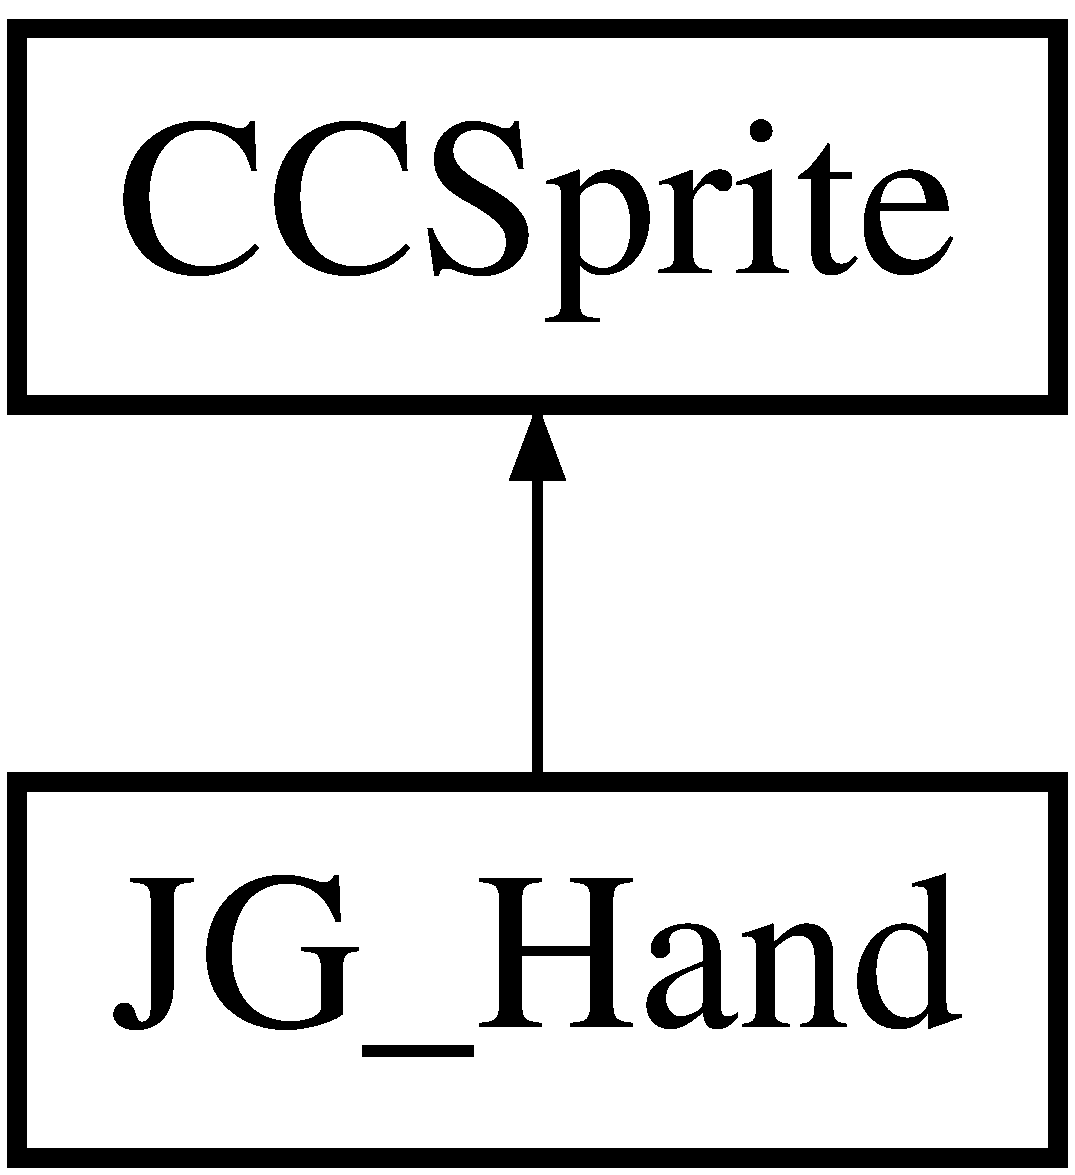
\includegraphics[height=2.000000cm]{class_j_g___hand}
\end{center}
\end{figure}
\subsection*{Public Member Functions}
\begin{DoxyCompactItemize}
\item 
\hypertarget{class_j_g___hand_aa66f82060cc53cf1790d2611476c76c0}{float {\bfseries Get\-Radius} ()}\label{class_j_g___hand_aa66f82060cc53cf1790d2611476c76c0}

\item 
\hypertarget{class_j_g___hand_aca220b8f6b4920e9324dd6b3e4f038ab}{{\bfseries C\-R\-E\-A\-T\-E\-\_\-\-F\-U\-N\-C} (\hyperlink{class_j_g___hand}{J\-G\-\_\-\-Hand})}\label{class_j_g___hand_aca220b8f6b4920e9324dd6b3e4f038ab}

\end{DoxyCompactItemize}
\subsection*{Static Public Member Functions}
\begin{DoxyCompactItemize}
\item 
\hypertarget{class_j_g___hand_af1e8c1afe129641193dc4f459ea3da62}{static \hyperlink{class_j_g___hand}{J\-G\-\_\-\-Hand} $\ast$ {\bfseries create\-With\-File\-Name} (const char $\ast$psz\-File\-Name, C\-C\-Point initial\-Pos)}\label{class_j_g___hand_af1e8c1afe129641193dc4f459ea3da62}

\end{DoxyCompactItemize}
\subsection*{Public Attributes}
\begin{DoxyCompactItemize}
\item 
\hypertarget{class_j_g___hand_abbebb5b5f2b897af0fa566477c817c96}{float {\bfseries radius}}\label{class_j_g___hand_abbebb5b5f2b897af0fa566477c817c96}

\end{DoxyCompactItemize}


The documentation for this class was generated from the following files\-:\begin{DoxyCompactItemize}
\item 
J\-G\-\_\-\-Hand.\-h\item 
J\-G\-\_\-\-Hand.\-cpp\end{DoxyCompactItemize}

\hypertarget{class_j_g___menu___main}{\section{J\-G\-\_\-\-Menu\-\_\-\-Main Class Reference}
\label{class_j_g___menu___main}\index{J\-G\-\_\-\-Menu\-\_\-\-Main@{J\-G\-\_\-\-Menu\-\_\-\-Main}}
}
Inheritance diagram for J\-G\-\_\-\-Menu\-\_\-\-Main\-:\begin{figure}[H]
\begin{center}
\leavevmode
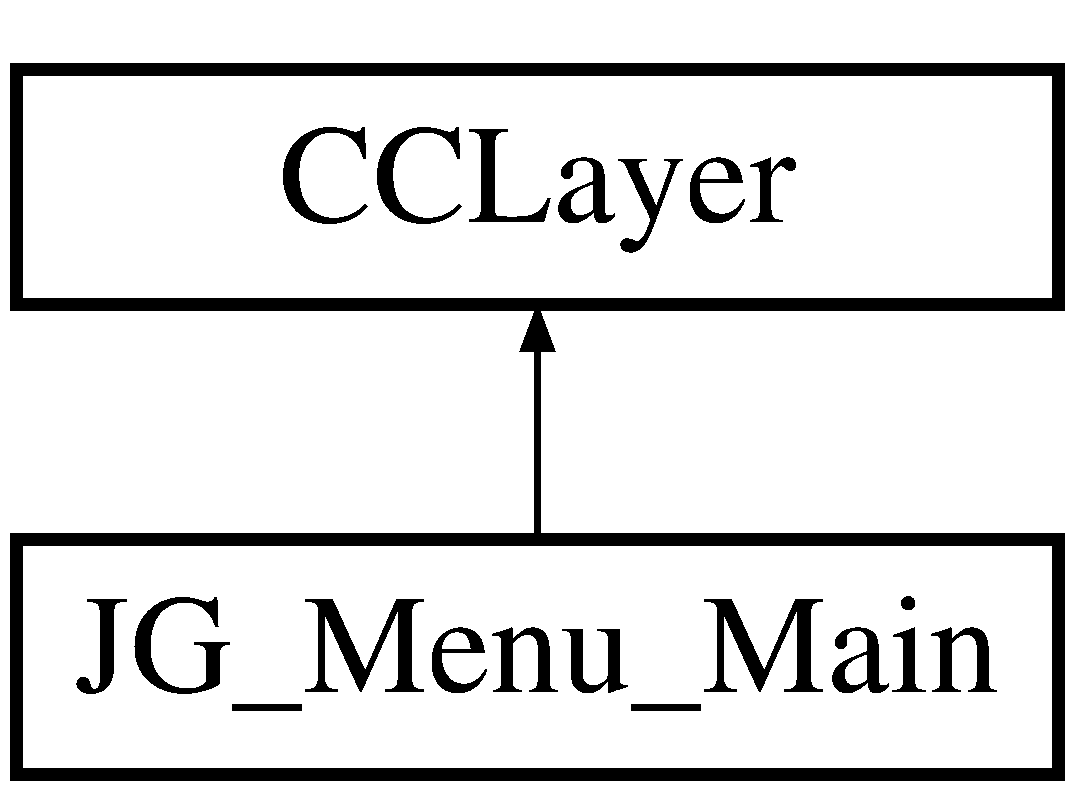
\includegraphics[height=2.000000cm]{class_j_g___menu___main}
\end{center}
\end{figure}
\subsection*{Public Member Functions}
\begin{DoxyCompactItemize}
\item 
\hypertarget{class_j_g___menu___main_ae015e299e7fd365043d747c6198cd418}{virtual bool {\bfseries init} ()}\label{class_j_g___menu___main_ae015e299e7fd365043d747c6198cd418}

\item 
\hypertarget{class_j_g___menu___main_aecbc239ff1644bff785af4e6a72dd516}{void {\bfseries menu\-Close\-Callback} (C\-C\-Object $\ast$p\-Sender)}\label{class_j_g___menu___main_aecbc239ff1644bff785af4e6a72dd516}

\item 
\hypertarget{class_j_g___menu___main_a606ffa5c67ae0d9451922ae2661583c8}{void {\bfseries menu\-Pause\-Call\-Back} (C\-C\-Object $\ast$p\-Sender)}\label{class_j_g___menu___main_a606ffa5c67ae0d9451922ae2661583c8}

\item 
\hypertarget{class_j_g___menu___main_a2abd1c8349ebb5469d4ea533abb69b51}{{\bfseries C\-R\-E\-A\-T\-E\-\_\-\-F\-U\-N\-C} (\hyperlink{class_j_g___menu___main}{J\-G\-\_\-\-Menu\-\_\-\-Main})}\label{class_j_g___menu___main_a2abd1c8349ebb5469d4ea533abb69b51}

\end{DoxyCompactItemize}
\subsection*{Static Public Member Functions}
\begin{DoxyCompactItemize}
\item 
\hypertarget{class_j_g___menu___main_a4725c05fccdb74b94d0b097e6310f743}{static cocos2d\-::\-C\-C\-Scene $\ast$ {\bfseries scene} ()}\label{class_j_g___menu___main_a4725c05fccdb74b94d0b097e6310f743}

\end{DoxyCompactItemize}


The documentation for this class was generated from the following files\-:\begin{DoxyCompactItemize}
\item 
J\-G\-\_\-\-Menu\-\_\-\-Main.\-h\item 
J\-G\-\_\-\-Menu\-\_\-\-Main.\-cpp\end{DoxyCompactItemize}

\hypertarget{struct_s_touch_info}{\section{S\-Touch\-Info Struct Reference}
\label{struct_s_touch_info}\index{S\-Touch\-Info@{S\-Touch\-Info}}
}
\subsection*{Public Attributes}
\begin{DoxyCompactItemize}
\item 
\hypertarget{struct_s_touch_info_a476c6db5c7f5ee0987fef6221fbceaf7}{C\-C\-Touch $\ast$ {\bfseries touch}}\label{struct_s_touch_info_a476c6db5c7f5ee0987fef6221fbceaf7}

\item 
\hypertarget{struct_s_touch_info_a354b68630606341541b282561bb4c292}{\hyperlink{class_j_g___hand}{J\-G\-\_\-\-Hand} $\ast$ {\bfseries hand}}\label{struct_s_touch_info_a354b68630606341541b282561bb4c292}

\item 
\hypertarget{struct_s_touch_info_aaed3c79798657884c11efa8a0e1fcb3f}{\hyperlink{class_j_g___ball}{J\-G\-\_\-\-Ball} $\ast$ {\bfseries ball}}\label{struct_s_touch_info_aaed3c79798657884c11efa8a0e1fcb3f}

\item 
\hypertarget{struct_s_touch_info_ab444619d360b1742837805506f9e1779}{bool {\bfseries b\-Is\-Dir\-Valid}}\label{struct_s_touch_info_ab444619d360b1742837805506f9e1779}

\item 
\hypertarget{struct_s_touch_info_a76f5cc268d81a4d3c80884669c7cc050}{float {\bfseries remaining\-Time}}\label{struct_s_touch_info_a76f5cc268d81a4d3c80884669c7cc050}

\item 
\hypertarget{struct_s_touch_info_ae1dd747adb4a406c03f18b5ffa45df6a}{C\-C\-Point {\bfseries initial\-Time\-Position}}\label{struct_s_touch_info_ae1dd747adb4a406c03f18b5ffa45df6a}

\end{DoxyCompactItemize}


The documentation for this struct was generated from the following file\-:\begin{DoxyCompactItemize}
\item 
J\-G\-\_\-\-Game\-\_\-\-Main.\-h\end{DoxyCompactItemize}

\hypertarget{structtag_resource}{\section{tag\-Resource Struct Reference}
\label{structtag_resource}\index{tag\-Resource@{tag\-Resource}}
}


The cocos2d Application.  




{\ttfamily \#include $<$App\-Delegate.\-h$>$}

\subsection*{Public Attributes}
\begin{DoxyCompactItemize}
\item 
\hypertarget{structtag_resource_a8640b003a8c5eef990ac1d0bd092c1c9}{cocos2d\-::\-C\-C\-Size {\bfseries size}}\label{structtag_resource_a8640b003a8c5eef990ac1d0bd092c1c9}

\item 
\hypertarget{structtag_resource_a347655ec02bf050e771cb4e6cb595537}{char {\bfseries directory} \mbox{[}100\mbox{]}}\label{structtag_resource_a347655ec02bf050e771cb4e6cb595537}

\end{DoxyCompactItemize}


\subsection{Detailed Description}
The cocos2d Application. 

The reason for implement as private inheritance is to hide some interface call by C\-C\-Director. 

The documentation for this struct was generated from the following file\-:\begin{DoxyCompactItemize}
\item 
App\-Delegate.\-h\end{DoxyCompactItemize}

%--- End generated contents ---

% Index
\newpage
\phantomsection
\addcontentsline{toc}{part}{Index}
\printindex

\end{document}
